% Created 2021-03-17 qua 17:49
% Intended LaTeX compiler: pdflatex
\documentclass{SelfArx}
  \usepackage[T1]{fontenc}
\usepackage[utf8]{inputenc}
\usepackage{booktabs}
\renewcommand{\arraystretch}{1.1} % Unclear
\usepackage{graphicx}
\usepackage{float}
\usepackage{amsmath}
\usepackage{csquotes}
\setlength{\fboxrule}{0.75pt} % Width of the border around the abstract
\definecolor{color1}{RGB}{0,0,90} % Color of the article title and sections
\definecolor{color2}{RGB}{0,20,20} % Color of the boxes behind the abstract and headings
\usepackage[portuguese, english]{babel} % Specify a different language here - english by default
\usepackage{lipsum} % Required to insert dummy text. To be removed otherwise
\usepackage[backend=biber,%
style = abnt,%
noslsn, %
isbn = false,
url = false,
extrayear, %
uniquename=init,%
giveninits, %
justify, %
sccite,%
scbib, %
sorting=nyt,
% mergedate=compact,
% natbib=true,
repeattitles, %
maxcitenames=3]{biblatex}
\AtEveryBibitem{%
\clearfield{urlyear}
\clearfield{urlmonth}
\clearfield{note}
\clearfield{issn} % Remove issn
\clearfield{doi} % Remove doi
\ifentrytype{online}{}{% Remove url except for @online
\clearfield{url}
}
}
\date{}
\title{Dados: O PIB da pandemia e cenários para 2021}
\begin{document}

\JournalInfo{Nota de Conjuntura No 16} % Journal information
\Archive{} % Additional notes (e.g. copyright, DOI, review/research article)

\Authors{Pedro Paulo Zahluth Bastos\textsuperscript{1}*, Lorena Dourado\textsuperscript{2}, Gabriel Petrini\textsuperscript{3}, Antônio Ibarra\textsuperscript{3}}} % Authors
\affiliation{\textsuperscript{1}\textit{Professor do Instituto de Economia Unicamp}} % Author affiliation
\affiliation{\textsuperscript{2}\textit{Graduanda do Instituto de Economia Unicamp}} % Author affiliation
\affiliation{\textsuperscript{3}\textit{Doutorando do Instituto de Economia  Unicamp}} % Author affiliation
\affiliation{*\textbf{E-mail}: ppzbastos@gmail.com} % Corresponding author

\Keywords{Keyword1 --- Keyword2 --- Keyword3} % Keywords - if you don't want any simply remove all the text between the curly brackets
\newcommand{\keywordname}{Palavras-chave} % Defines the keywords heading name

\Abstract{
\begin{itemize}

\item Em março, havia risco de sucessão longa de quedas trimestrais do PIB, com círculo vicioso de contração de demanda, contração do crédito, falências de empresas e ampliação do desemprego e da pobreza.
\item O risco foi contornado com política anticíclica para sustentar renda, vínculos empregatícios e, tardiamente, ampliação do crédito (apesar do repasse da depreciação cambial).
\item A continuidade da pandemia limitou a retomada da demanda e do emprego em serviços em razão do risco de contágio, reafirmando a centralidade do controle da pandemia para a recuperação da economia (não há trade-off duradouro).
\item A magnitude da política anticíclica gera um risco enorme de um segundo mergulho em razão da retomada da lei do teto do gasto e da retirada brusca dos programas emergenciais.
\item Sem política anticíclica, aumento do desemprego e da pobreza serão dramáticos ainda que as exportações se recuperem em 2021.
\end{itemize}
}
\renewcommand{\abstractname}{Sumário Executivo} % Defines the keywords heading name
\flushbottom % Makes all text pages the same height
\maketitle % Print the title and abstract box
\thispagestyle{empty} % Removes page numbering from the first page
\onecolumn

\section*{Indicadores de antecedente}
\label{sec:org6ba496f}
\subsection*{IBC-Br (acumulado 12 meses vs 12 meses anteriores)}
\label{sec:org2603bf3}

\begin{center}
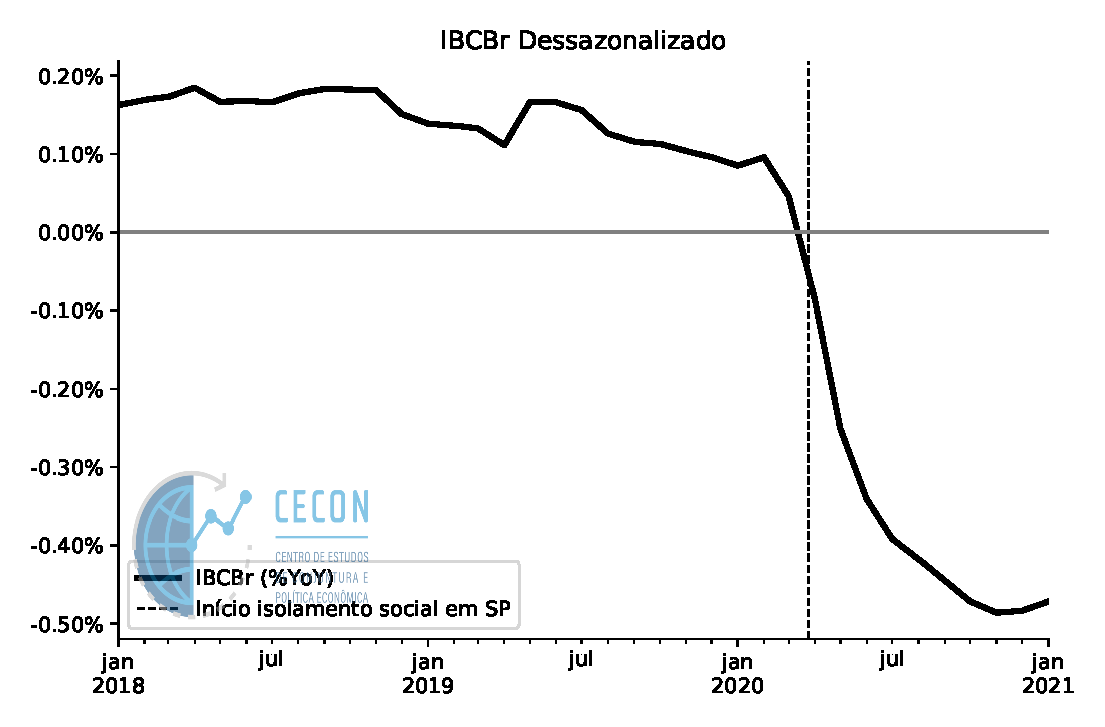
\includegraphics[width=.9\linewidth]{./figs/Antecedente/IBCBr.pdf}
\end{center}

\subsection*{Tráfego de veículos pesados nas estradas pedagiadas - ABCR - Dados dessazonalizados}
\label{sec:orged63d87}


\begin{center}
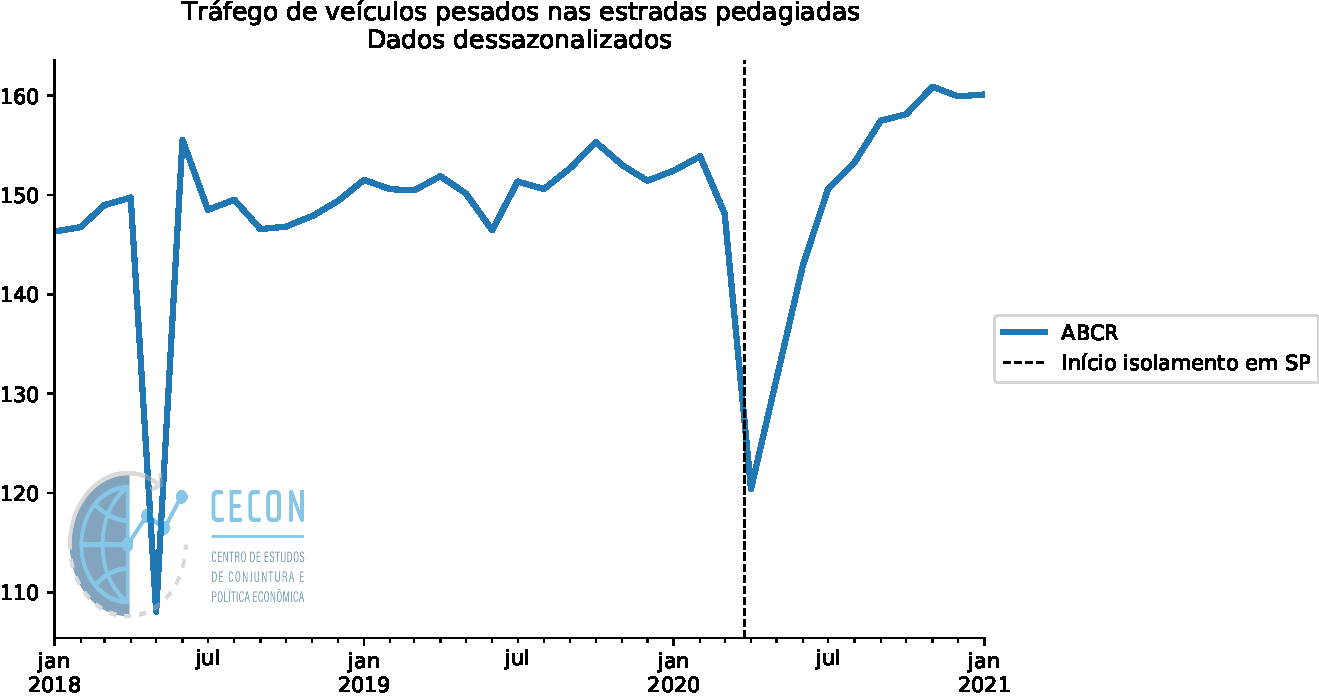
\includegraphics[width=.9\linewidth]{./figs/Setoriais/TrafegoPedagio.pdf}
\end{center}


\section*{Dados de alta frequência}
\label{sec:org478e175}

\subsection*{Bloomberg adaptado ao COVID-19 (\href{https://www.bloomberg.com/news/articles/2020-11-13/alternative-data-show-activity-crashes-as-virus-resurges-chart}{Link})}
\label{sec:org5f1052a}

\subsection*{Google Reports: Brasil}
\label{sec:orgd0db10d}

\begin{center}
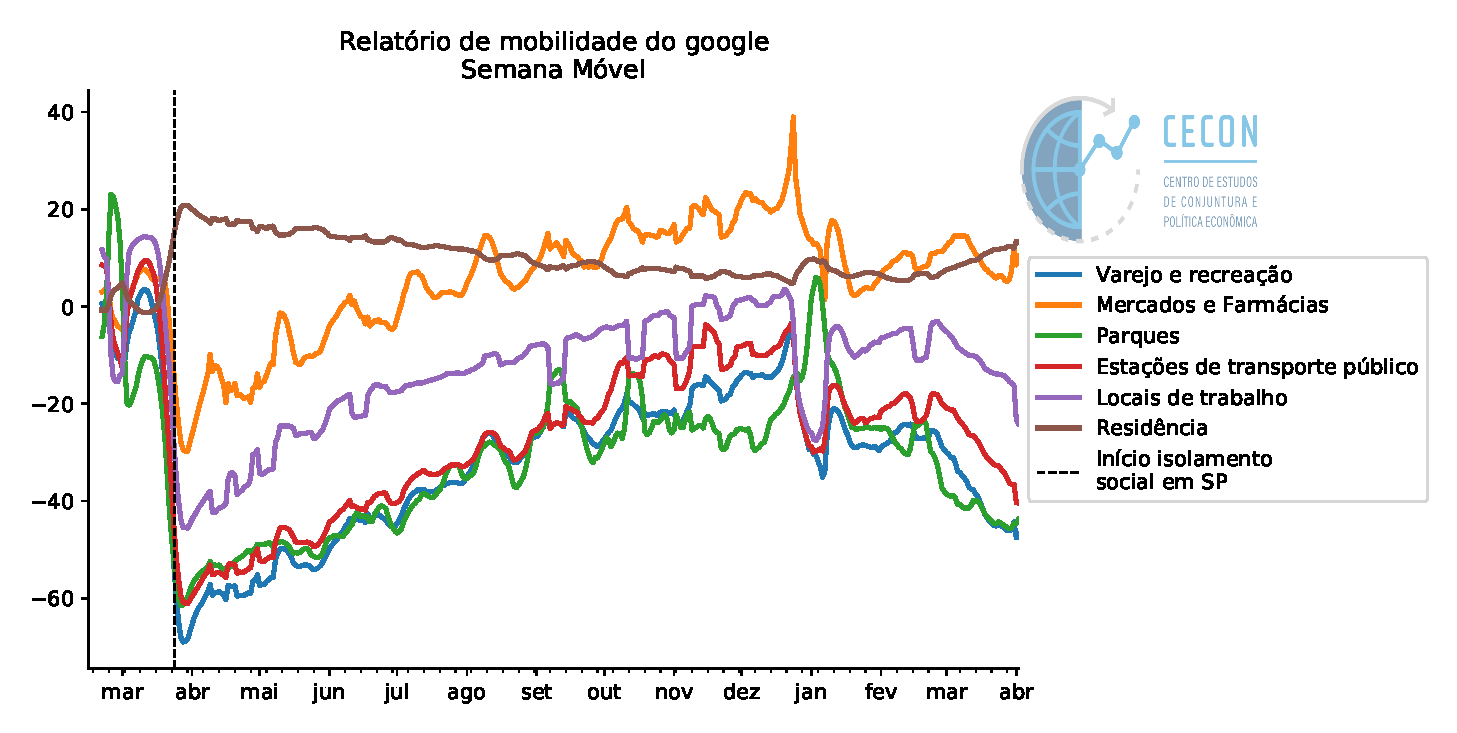
\includegraphics[width=.9\linewidth]{./figs/Granulares/GoogleReport_Brasil.pdf}
\end{center}

\subsection*{Apple: Tendências de mobilidade}
\label{sec:org4c6e832}

\begin{center}
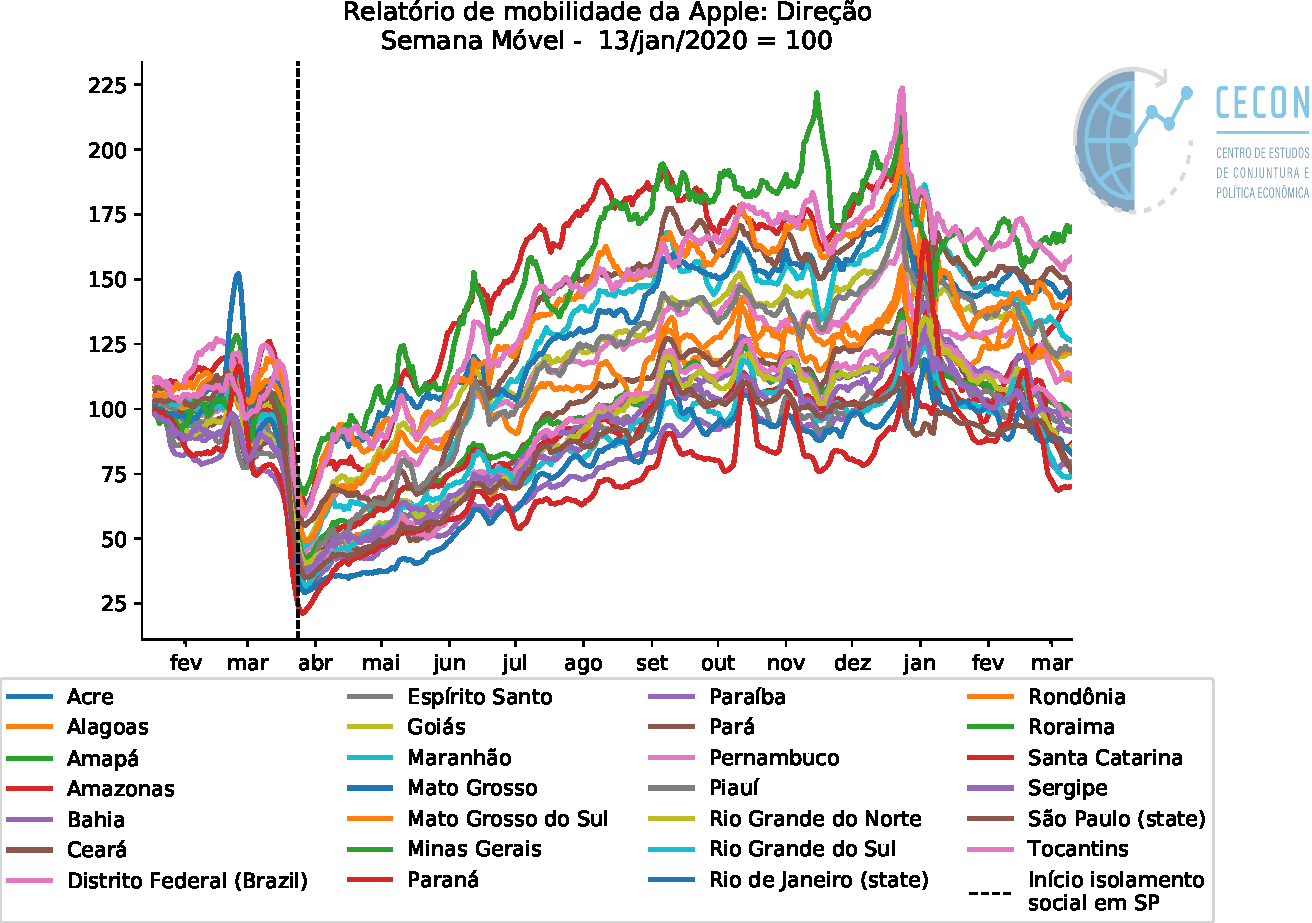
\includegraphics[width=.9\linewidth]{./figs/Granulares/AppleReport_Brasil.pdf}
\end{center}

\subsection*{Waze: \(\Delta \%\) Km}
\label{sec:org7082e49}

\begin{center}
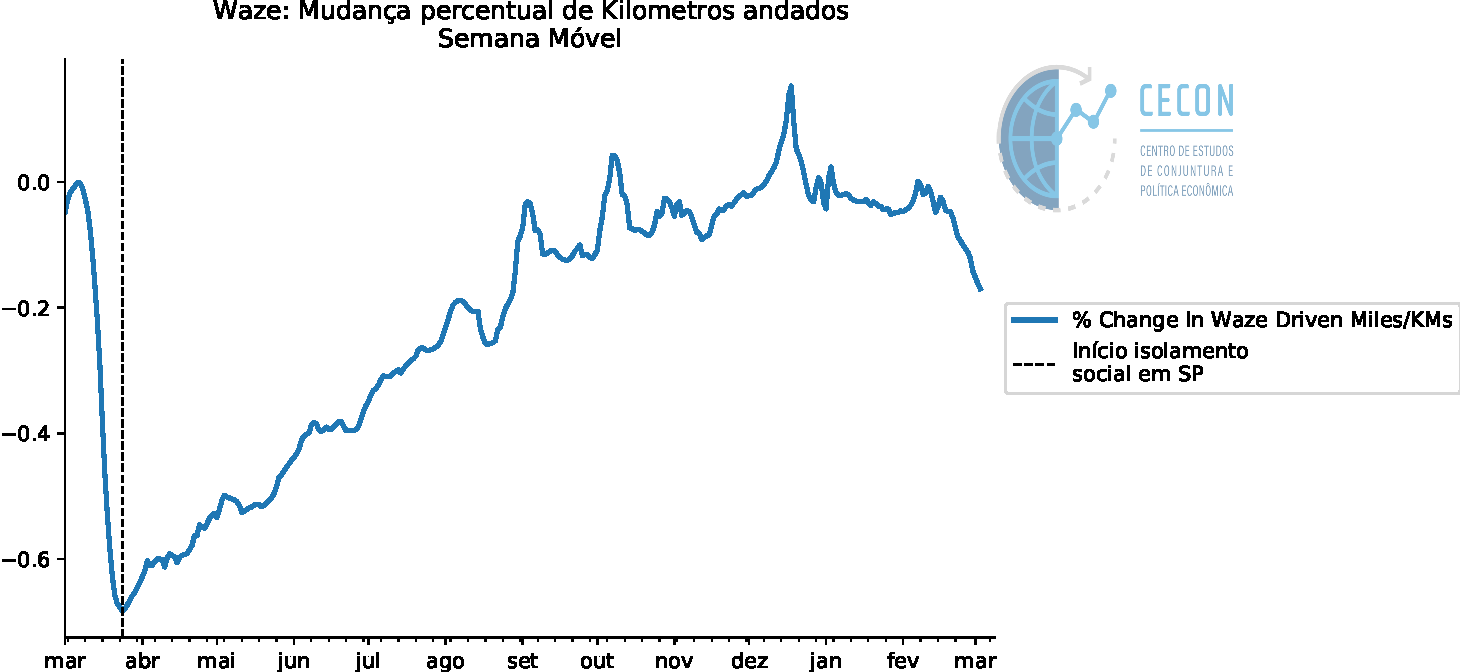
\includegraphics[width=.9\linewidth]{./figs/Granulares/Waze_Brasil.pdf}
\end{center}

\subsection*{TomTom: Congestionamento}
\label{sec:org8e88253}

\begin{center}
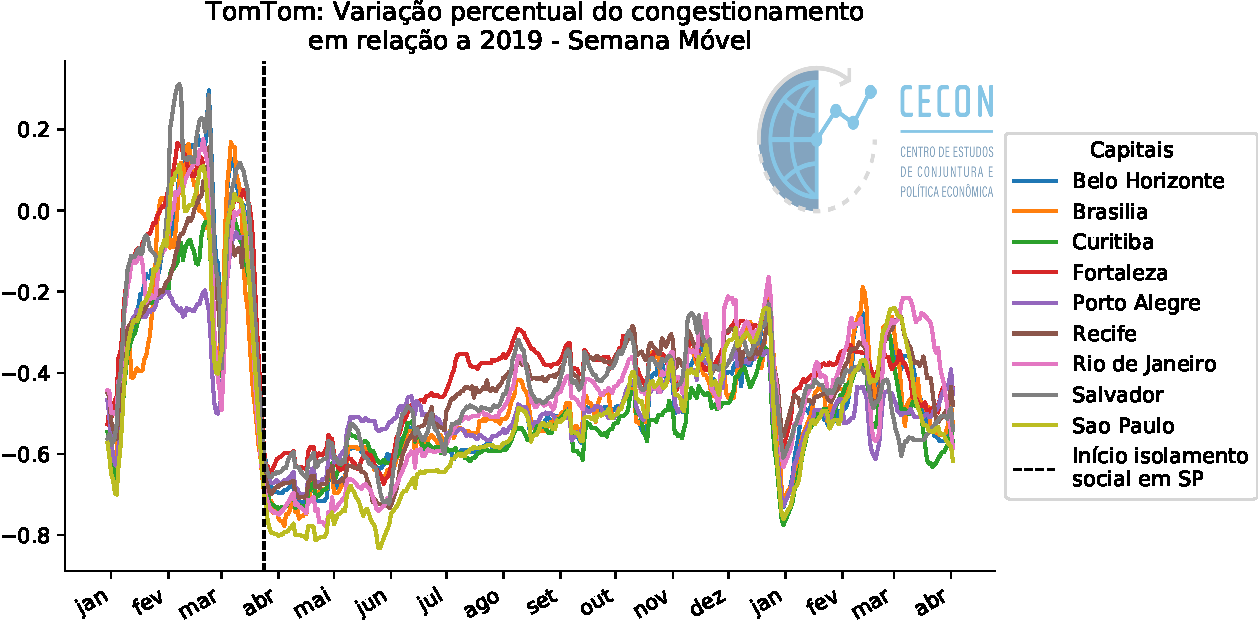
\includegraphics[width=.9\linewidth]{./figs/Granulares/TomTom_Brasil.pdf}
\end{center}

\section*{Atividade}
\label{sec:orge9adff7}



\subsection*{Trimestre Contra trimestre imediatamente anterior}
\label{sec:orgede3a23}

\begin{center}
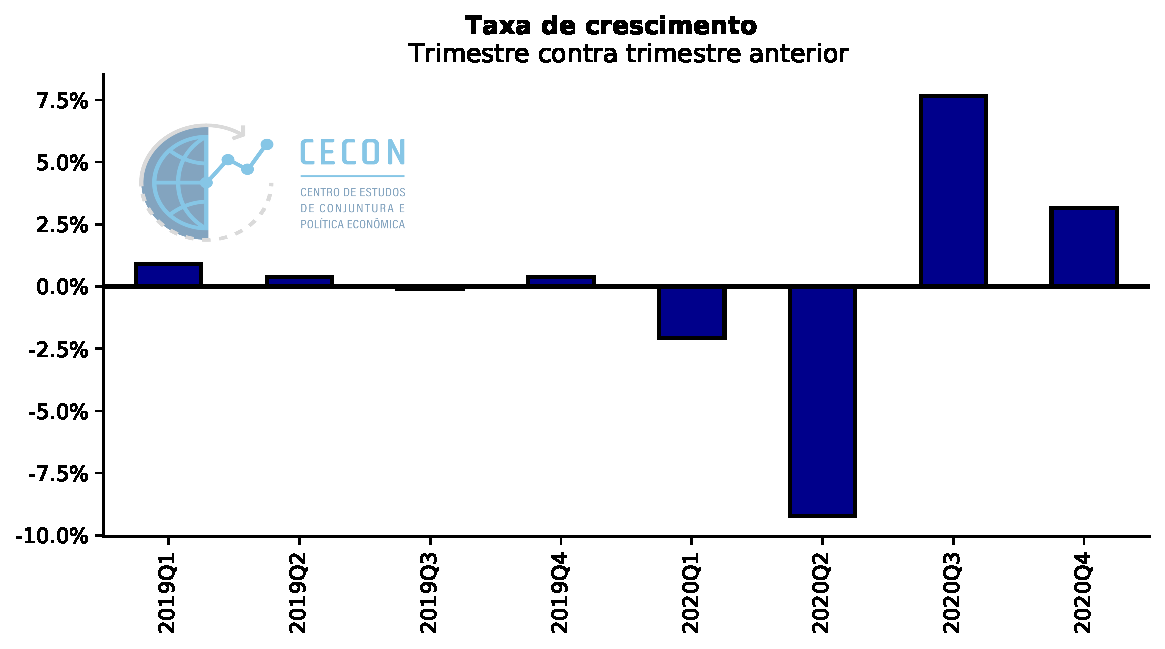
\includegraphics[width=.9\linewidth]{./figs/PIB/PIB.pdf}
\end{center}

\subsection*{Trimestre Contra mesmo trimestre do ano anterior}
\label{sec:org18e864b}

\begin{center}
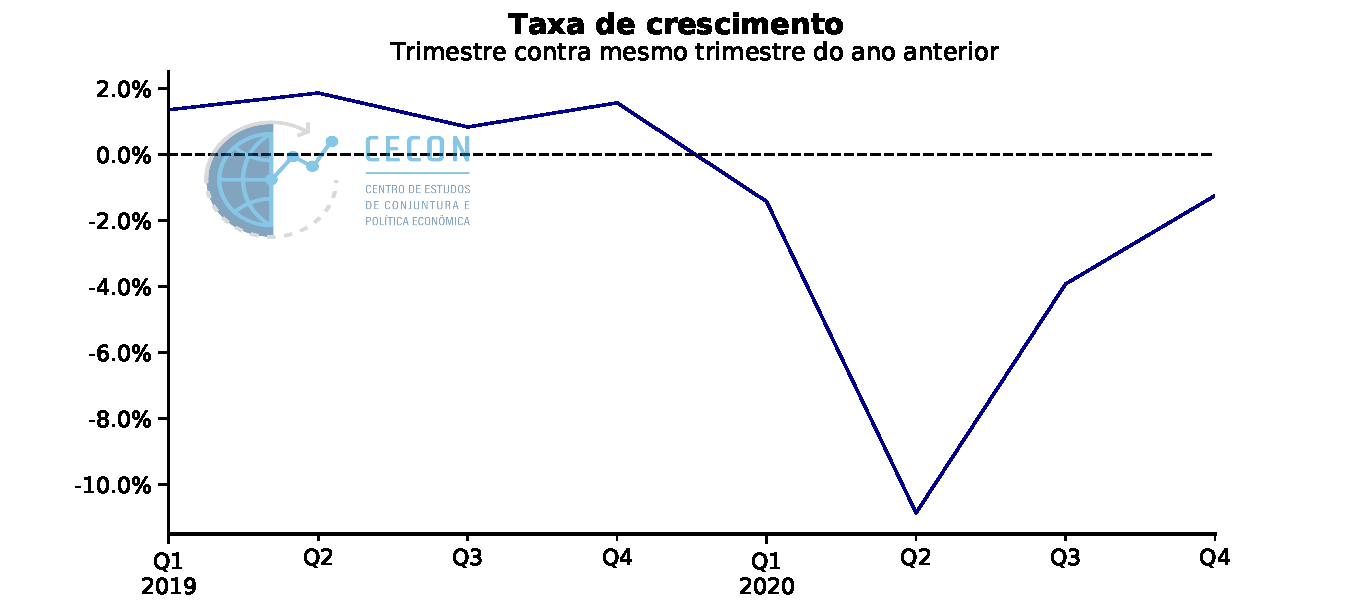
\includegraphics[width=.9\linewidth]{./figs/PIB/PIB_YoY.pdf}
\end{center}

\subsection*{Agropecuária}
\label{sec:orgc3f84e6}

\begin{center}
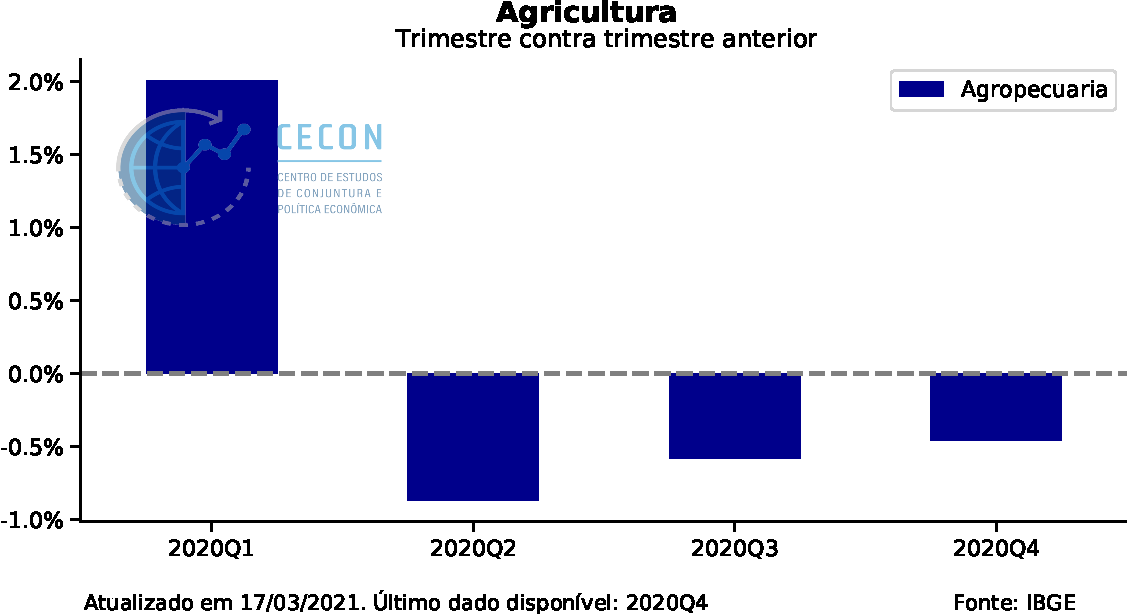
\includegraphics[width=.9\linewidth]{./figs/PIB/Agropecuaria.pdf}
\end{center}

\subsection*{Indústria}
\label{sec:orgf9909b1}

\begin{center}
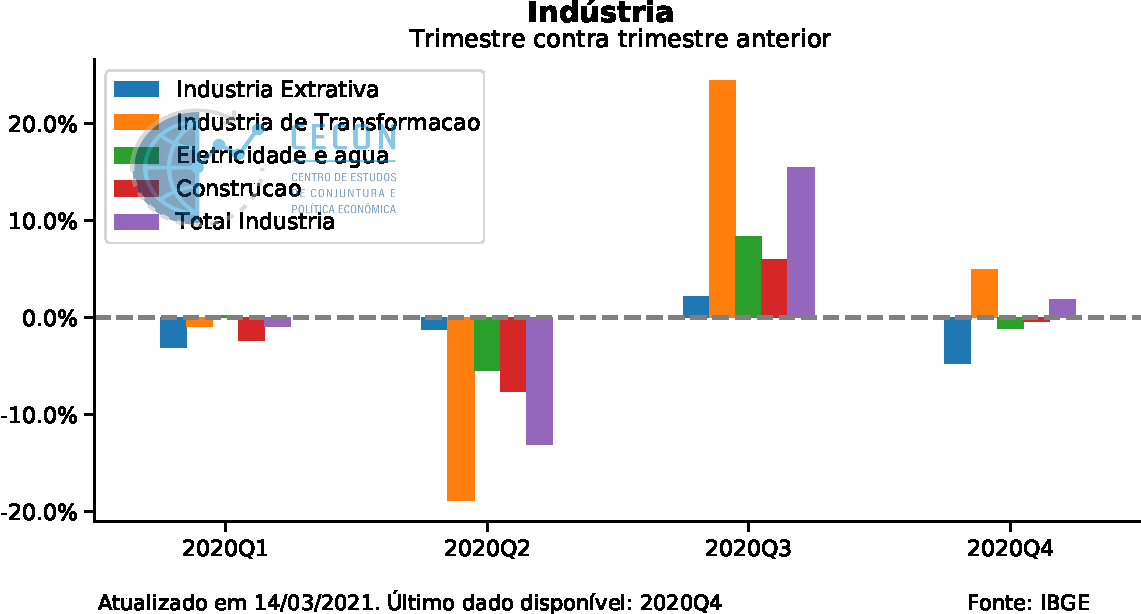
\includegraphics[width=.9\linewidth]{./figs/PIB/Industria.pdf}
\end{center}


\subsection*{Serviços}
\label{sec:org29ece94}

\begin{center}
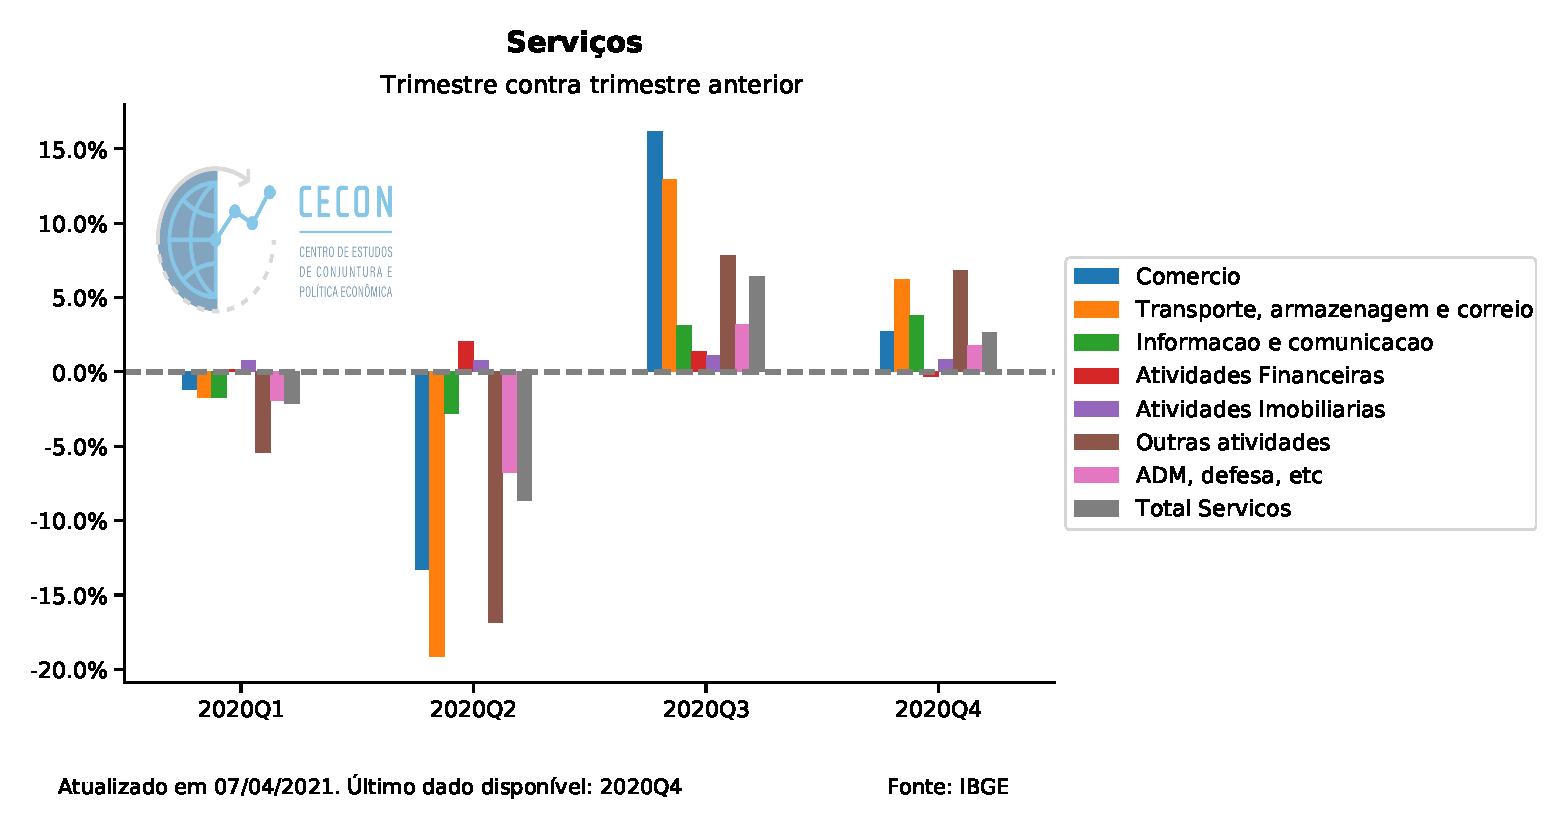
\includegraphics[width=.9\linewidth]{./figs/PIB/Servicos.pdf}
\end{center}

\subsection*{Demanda}
\label{sec:orgc8396ab}

\begin{center}
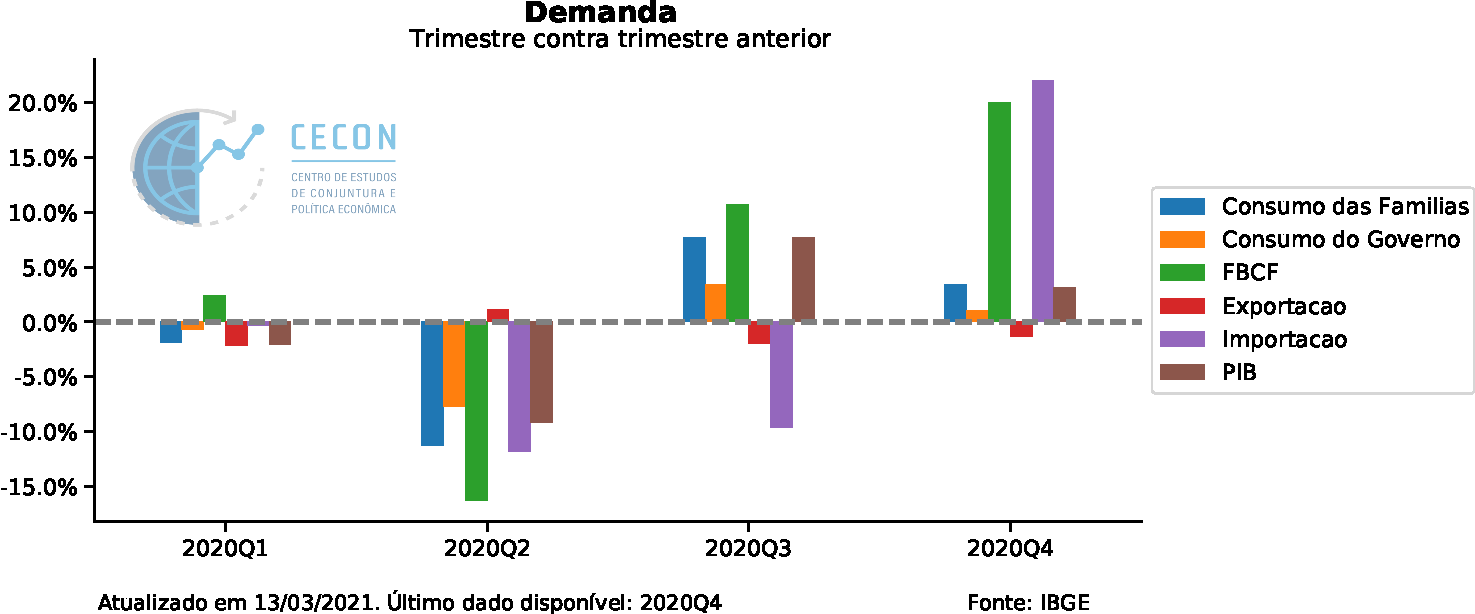
\includegraphics[width=.9\linewidth]{./figs/PIB/Demanda.pdf}
\end{center}

\subsection*{Oferta}
\label{sec:org8c09234}


\begin{center}
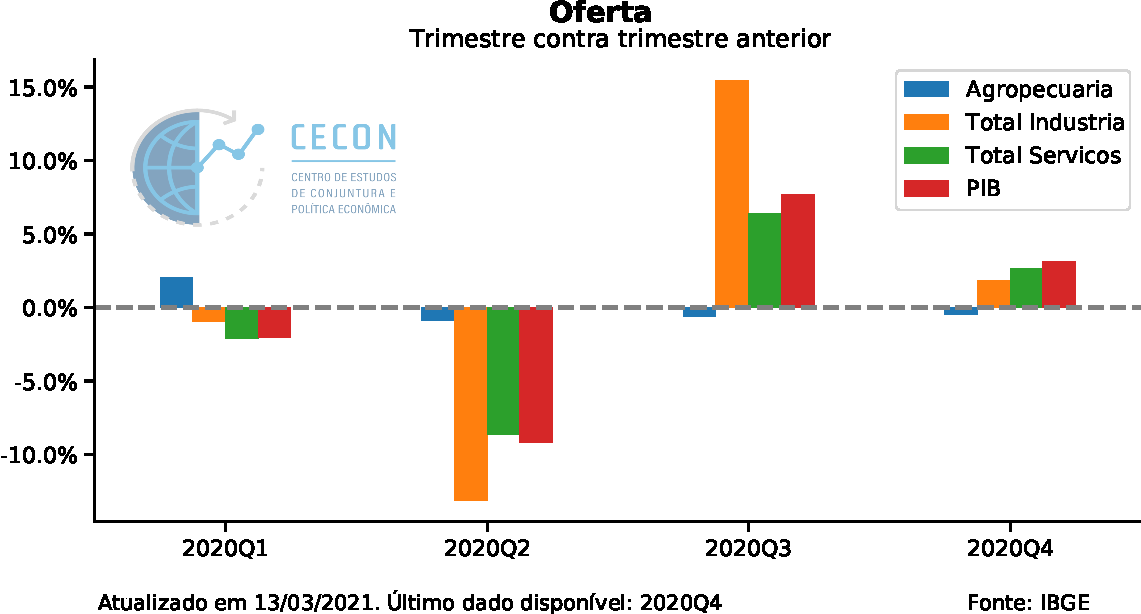
\includegraphics[width=.9\linewidth]{./figs/PIB/Oferta.pdf}
\end{center}


\subsection*{Contribuição para variação: Demanda}
\label{sec:org860b95b}

\begin{center}
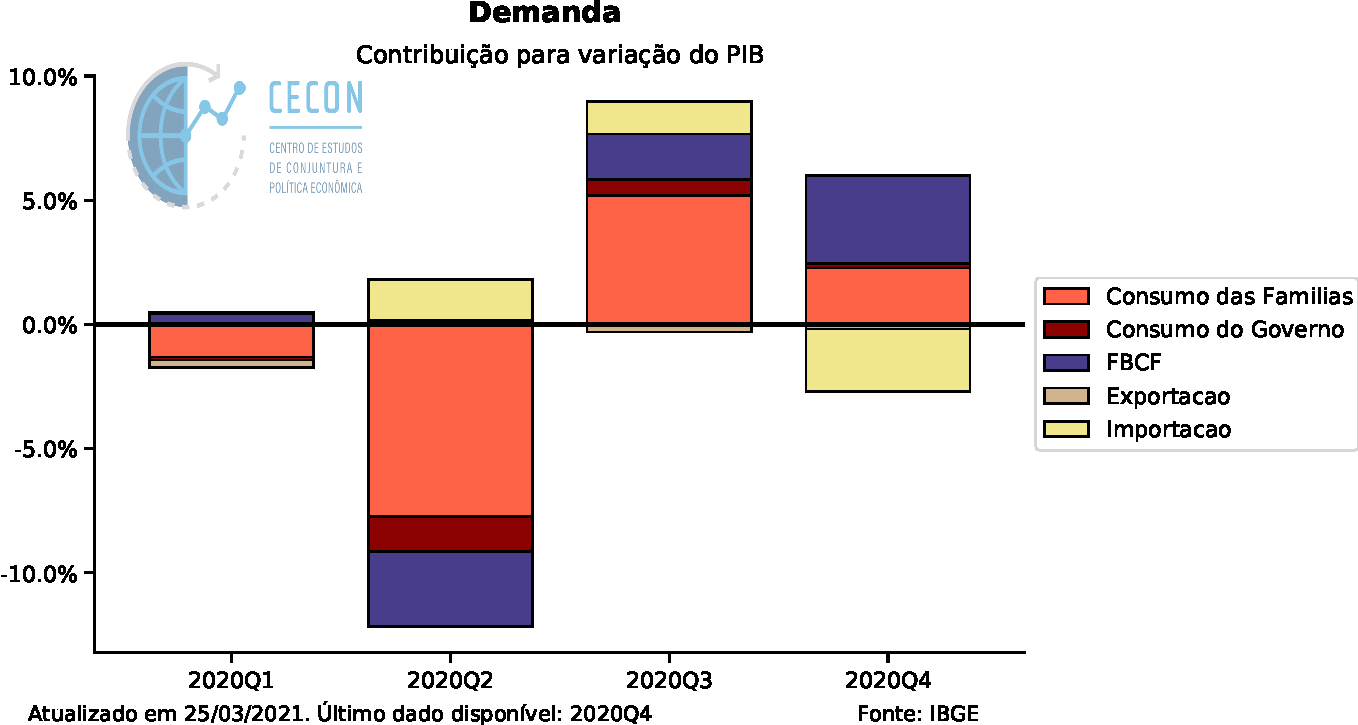
\includegraphics[width=.9\linewidth]{./figs/PIB/Contrib_Demanda.pdf}
\end{center}

\subsection*{Contribuição para variação: Oferta}
\label{sec:org85fc674}

\begin{center}
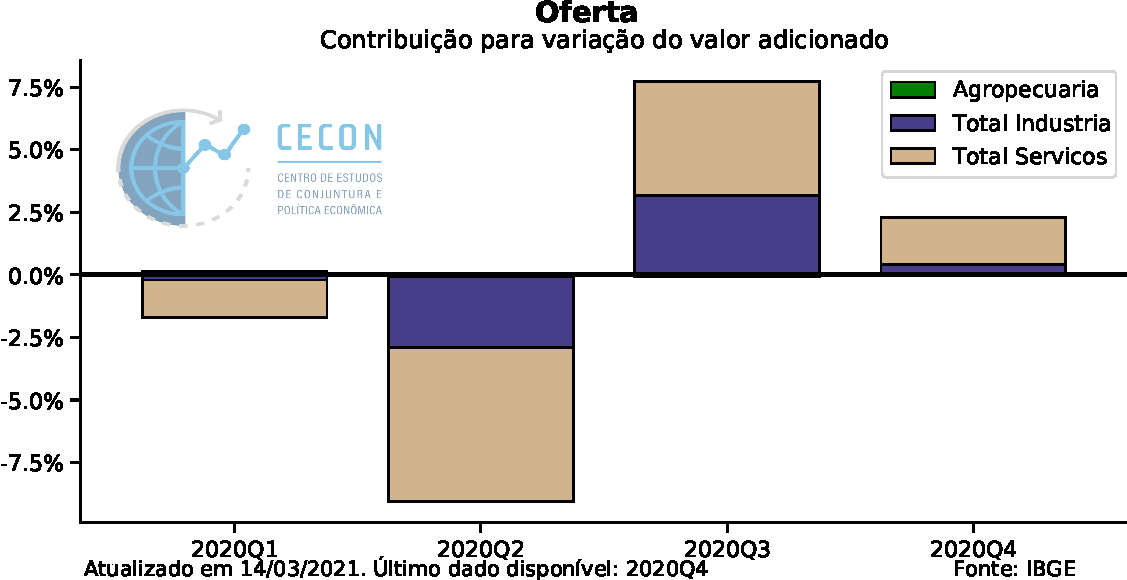
\includegraphics[width=.9\linewidth]{./figs/PIB/Contrib_Oferta.pdf}
\end{center}


\subsection*{Contribuição para variação: Serviços}
\label{sec:org72427d0}

\begin{center}
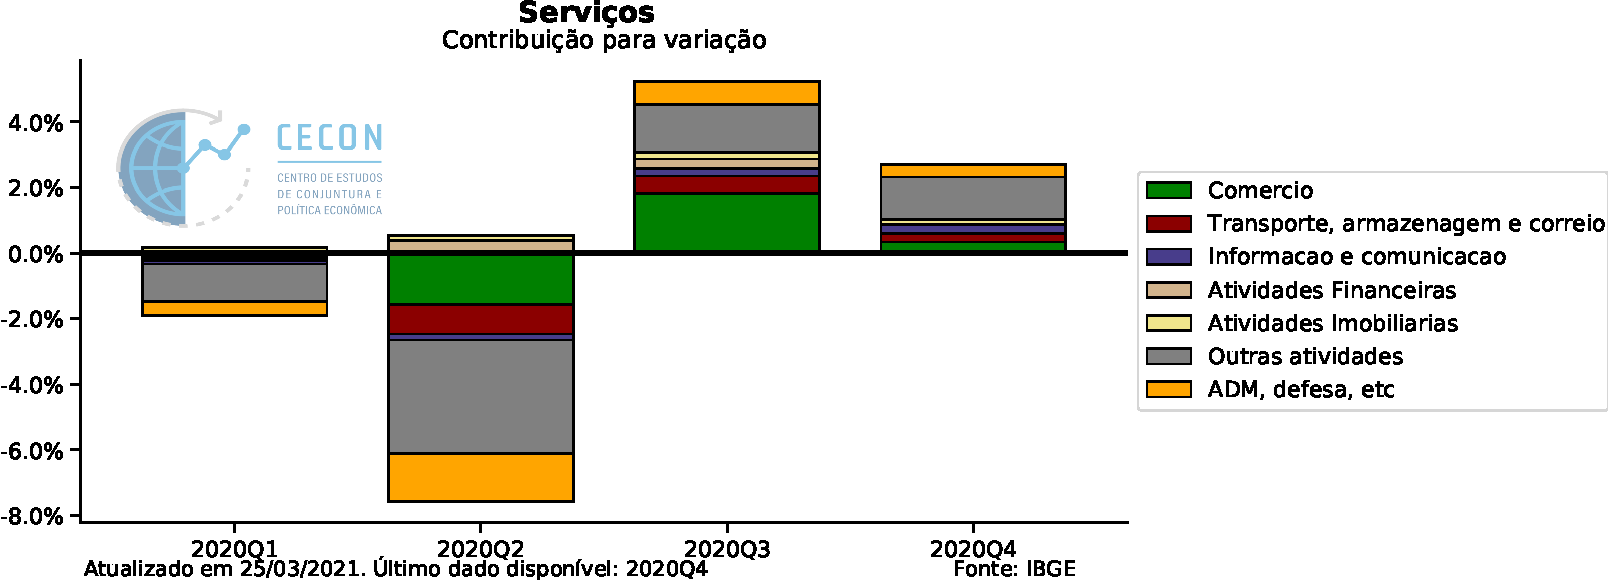
\includegraphics[width=.9\linewidth]{./figs/PIB/Contrib_Servicos.pdf}
\end{center}

\subsection*{Acumulado no ano (sem ajuste)}
\label{sec:org7a2fdc9}

\subsubsection*{Serviços}
\label{sec:orgd1caaa6}

\begin{center}
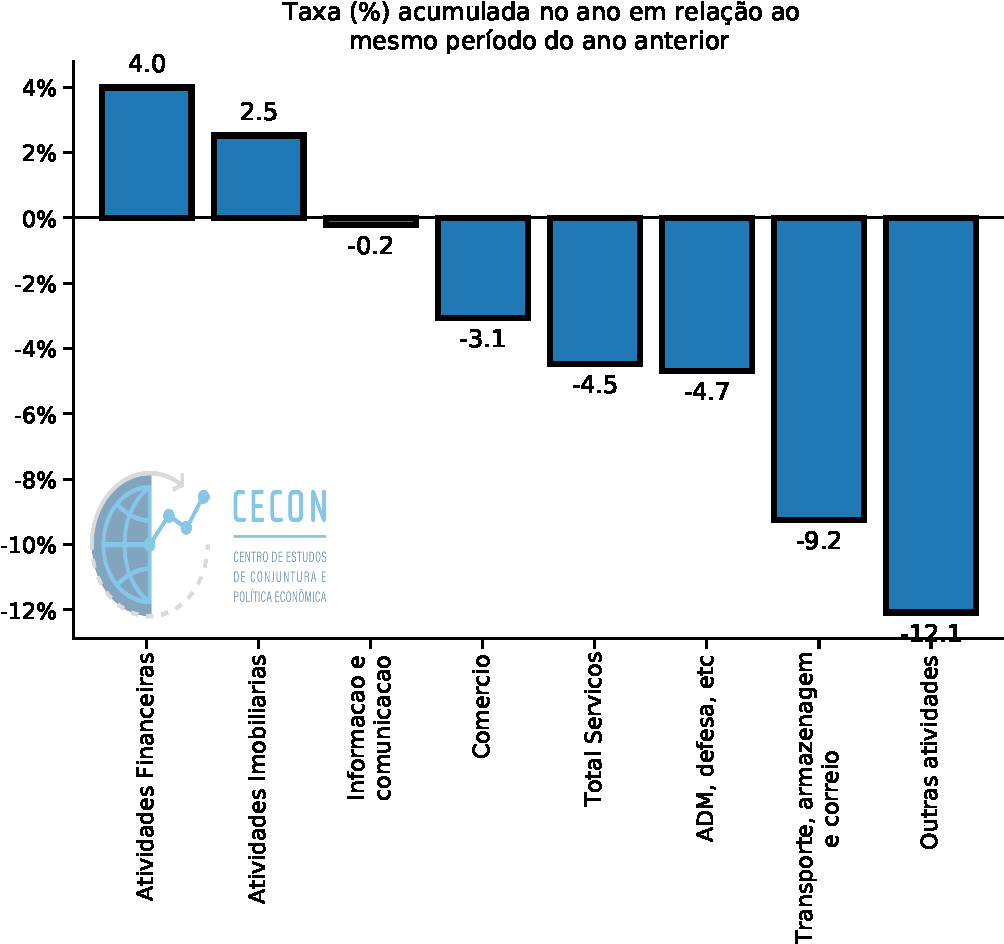
\includegraphics[width=.9\linewidth]{./figs/PIB/Servicos_Acum.pdf}
\end{center}

\subsubsection*{Serviços (comparação com ano anterior)}
\label{sec:org8bfae64}

\begin{center}
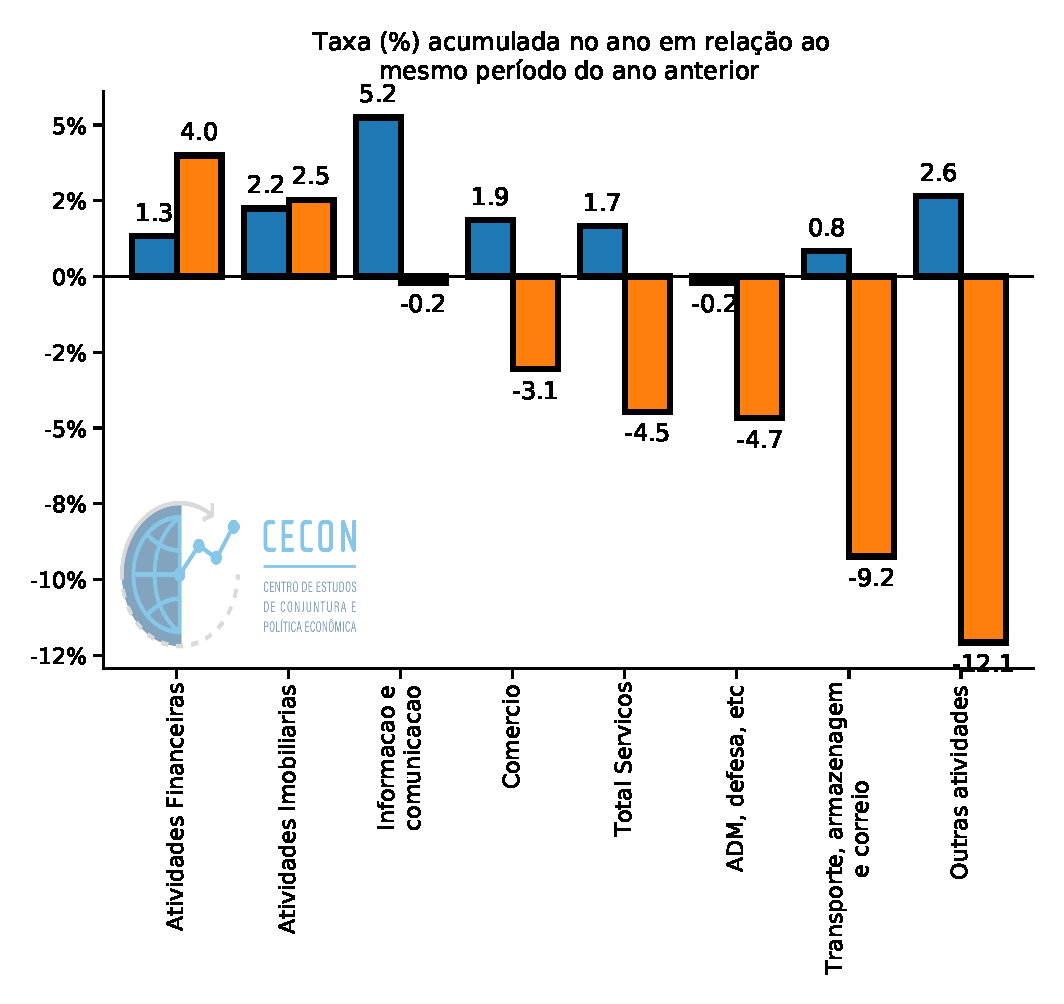
\includegraphics[width=.9\linewidth]{./figs/PIB/Servicos_Acum_Comparativo.pdf}
\end{center}

\subsubsection*{Demanda}
\label{sec:org9dfa3bf}

\begin{center}
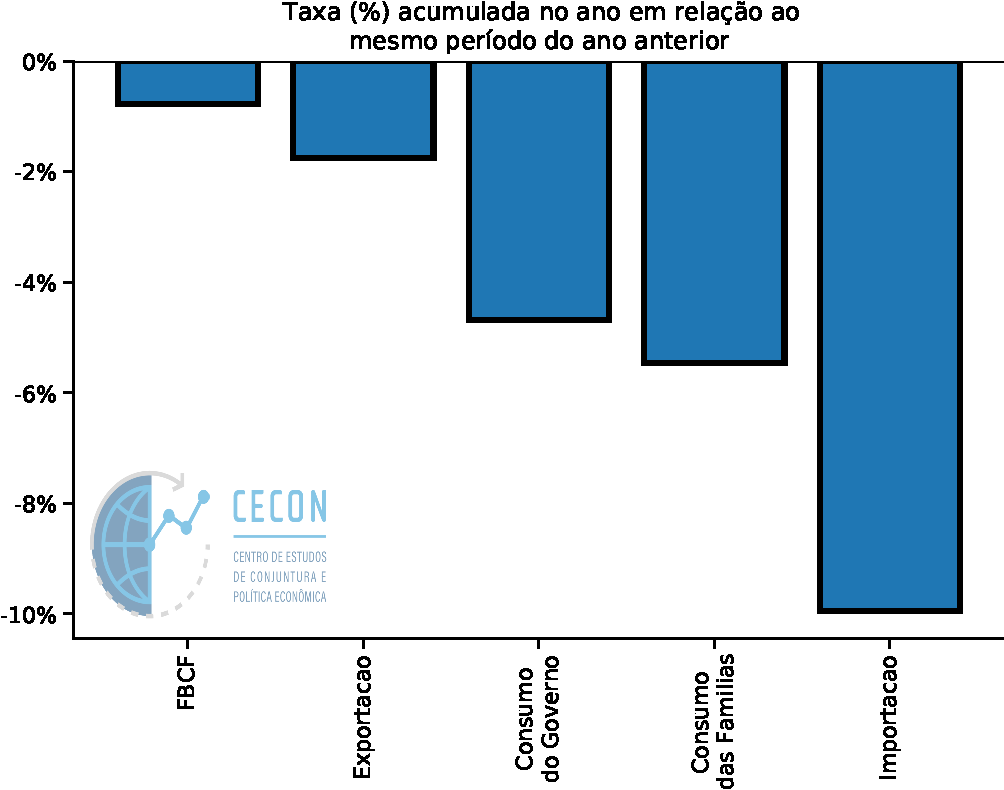
\includegraphics[width=.9\linewidth]{./figs/PIB/Demanda_Acum.pdf}
\end{center}

\subsubsection*{Demanda (comparação com ano anterior)}
\label{sec:org4c7e7e2}

\begin{center}
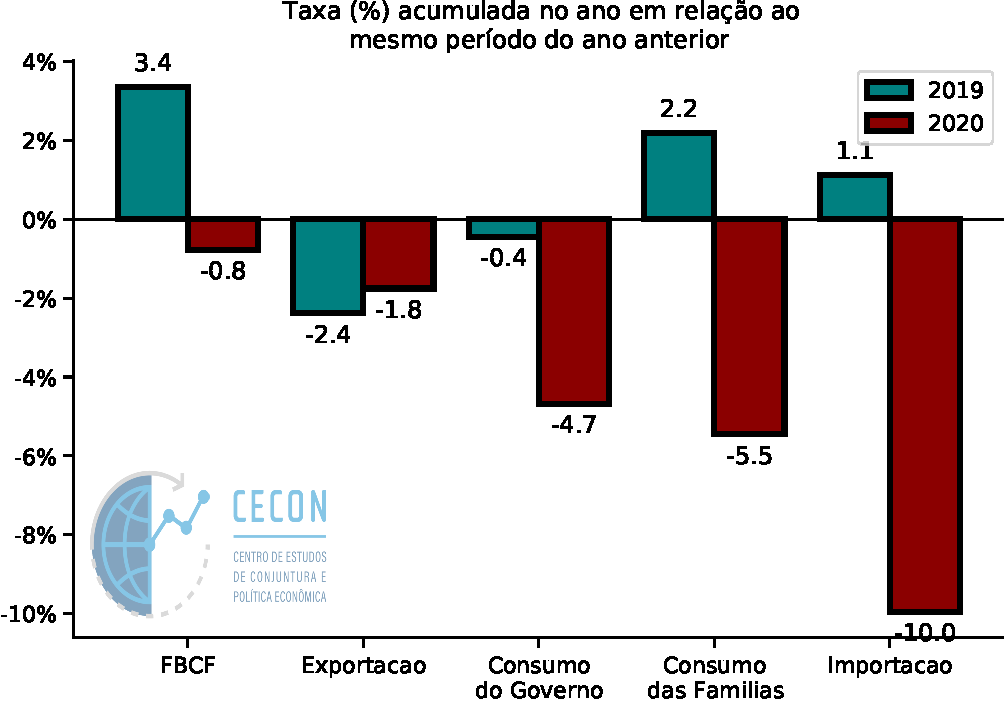
\includegraphics[width=.9\linewidth]{./figs/PIB/Demanda_Acum_Comparativo.pdf}
\end{center}

\section*{Crédito}
\label{sec:org1742389}

\subsection*{Endividamento das famílias}
\label{sec:org02a6b80}

\begin{center}
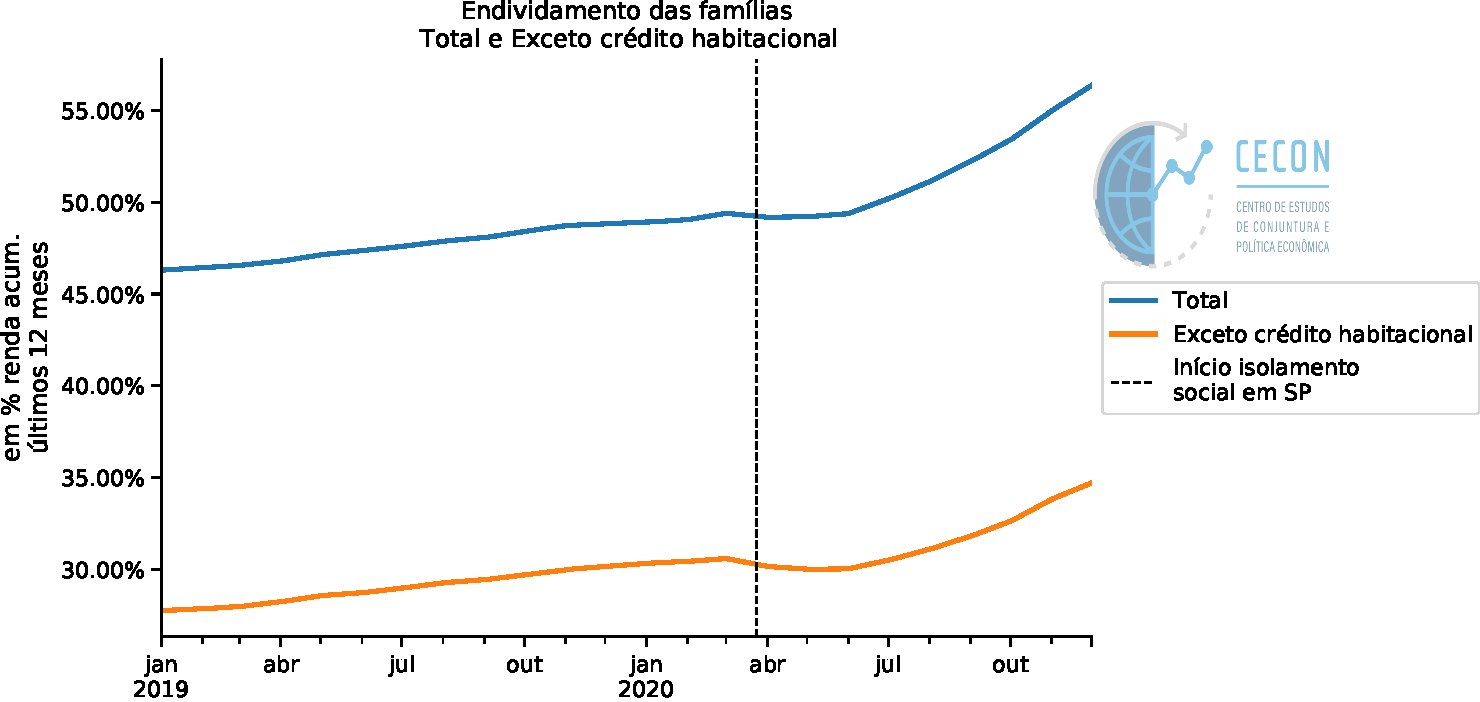
\includegraphics[width=.9\linewidth]{./figs/Credito/EndividamentoFamilias.pdf}
\end{center}


\subsection*{Saldo Pessoal Jurídica - Nível}
\label{sec:org80b9b00}

\begin{center}
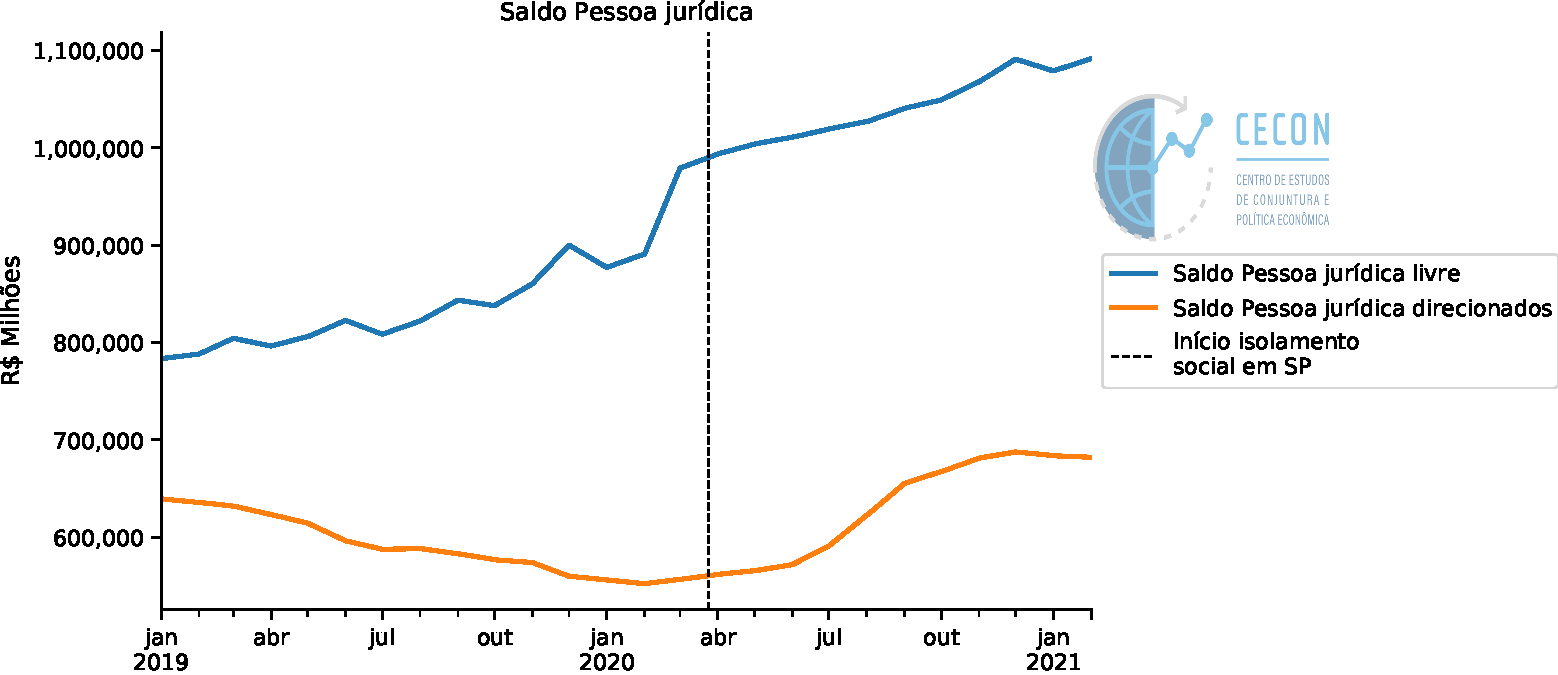
\includegraphics[width=.9\linewidth]{./figs/Credito/SaldoPJ.pdf}
\end{center}



\subsection*{Saldo Pessoa Jurídica - em \% do PIB}
\label{sec:orgfac5201}
\begin{center}
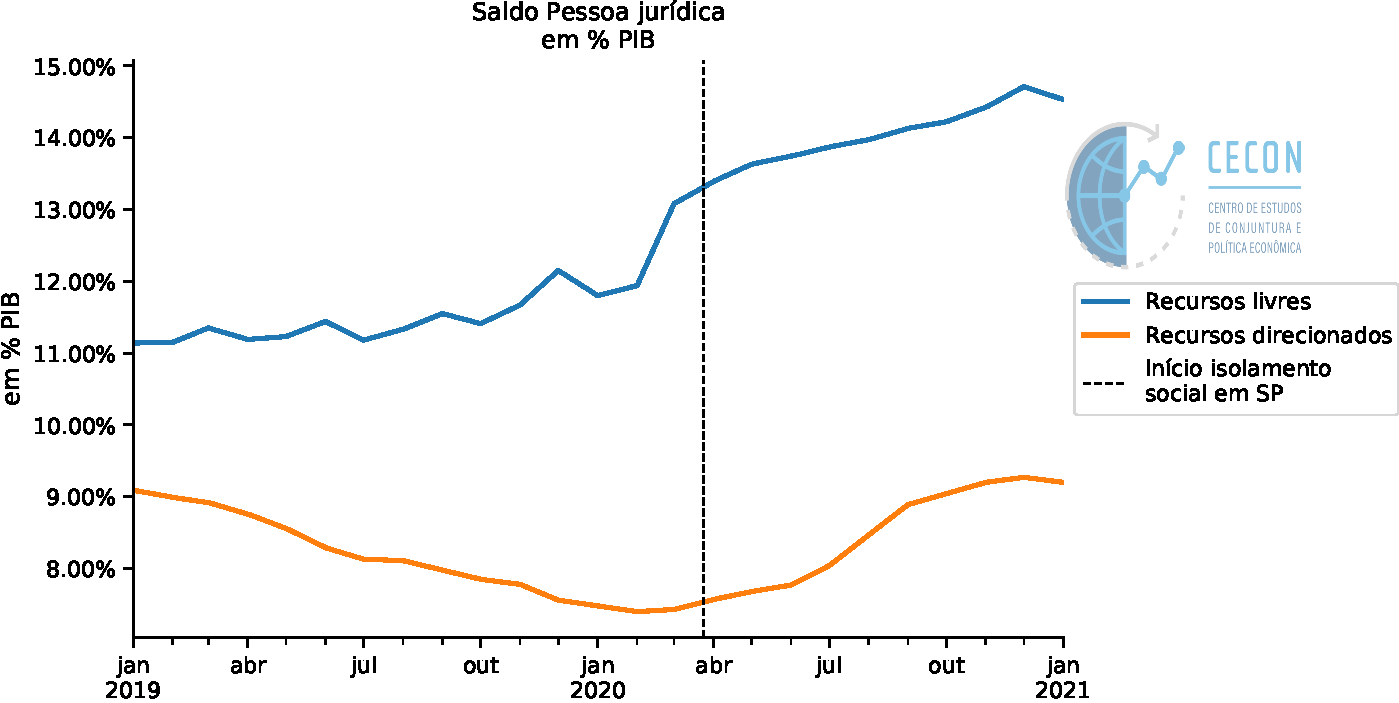
\includegraphics[width=.9\linewidth]{./figs/Credito/SaldoPJ_PIB.pdf}
\end{center}

\subsection*{Saldo Pessoa física - Nível}
\label{sec:org000f177}

\begin{center}
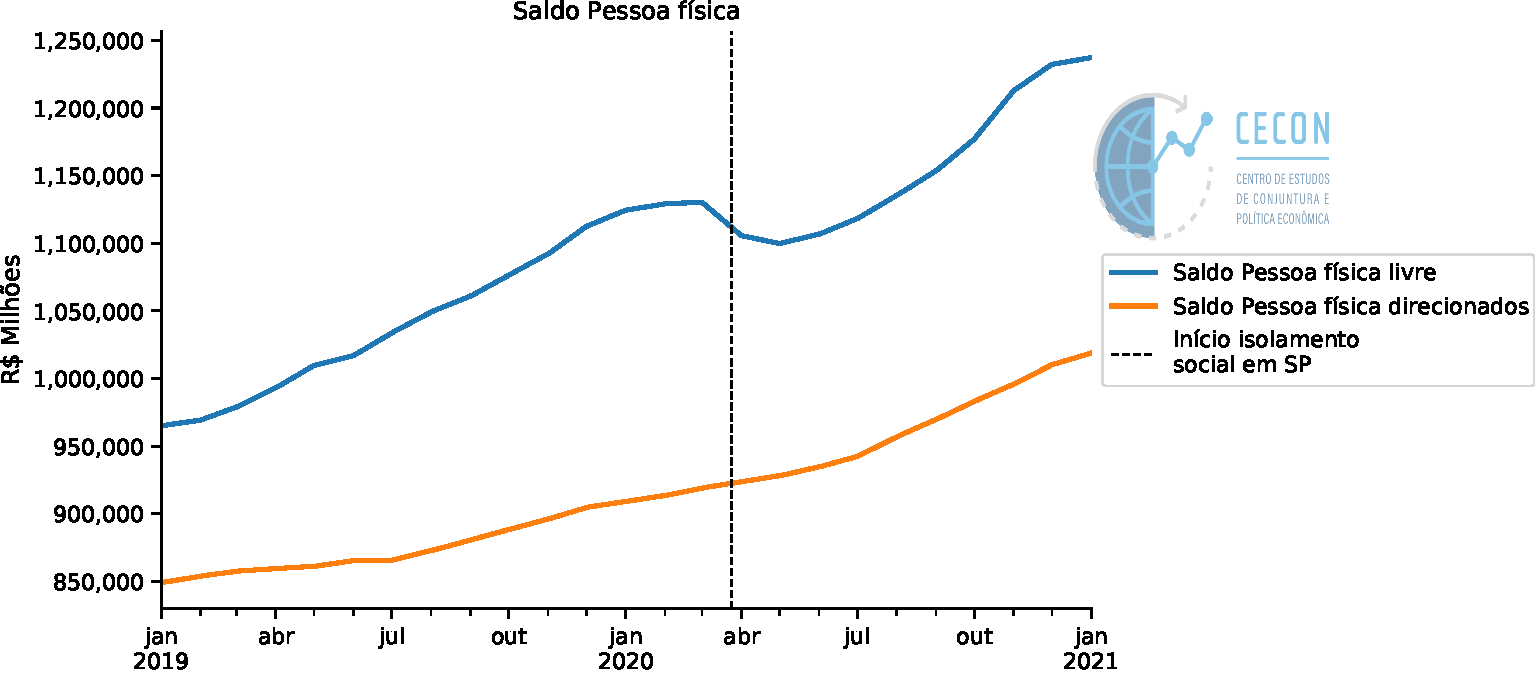
\includegraphics[width=.9\linewidth]{./figs/Credito/SaldoPF.pdf}
\end{center}


\subsection*{Saldo Pessoa física - em \% do PIB}
\label{sec:orgcf5ef6d}

\begin{center}
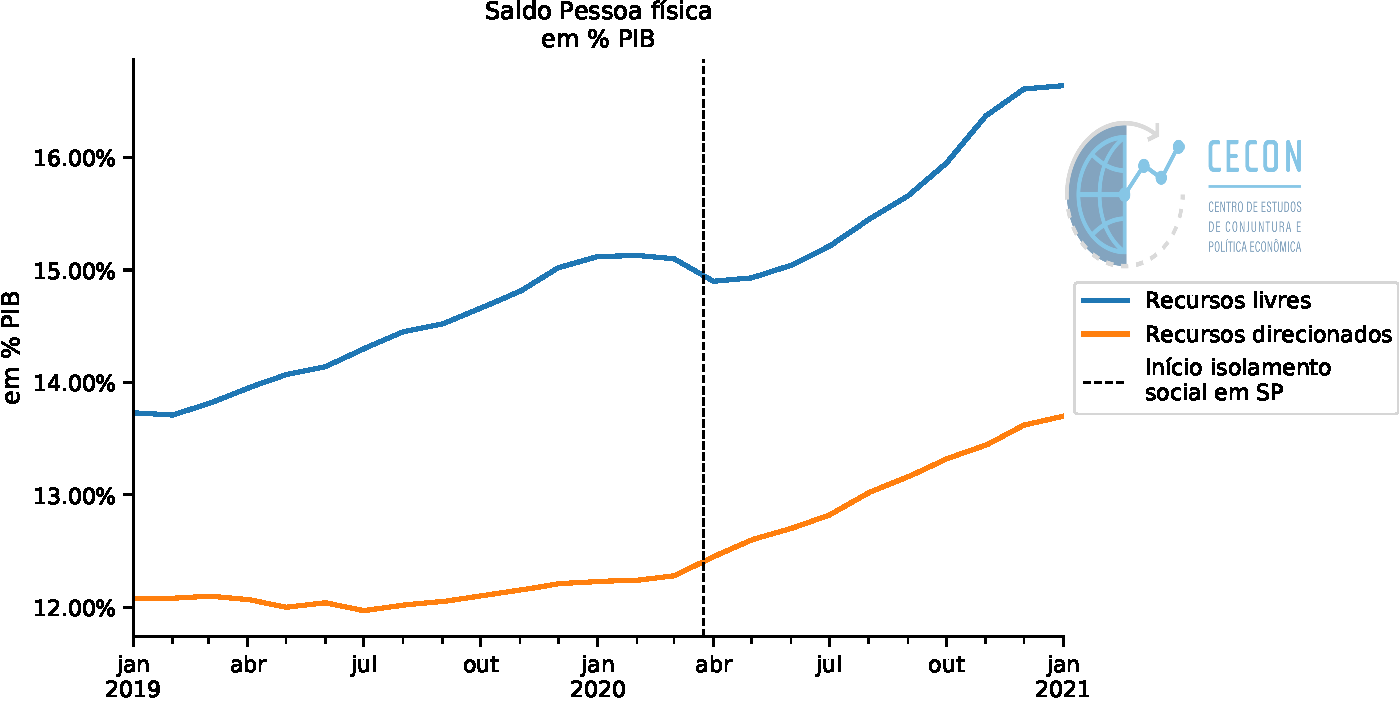
\includegraphics[width=.9\linewidth]{./figs/Credito/SaldoPF_PIB.pdf}
\end{center}


\subsection*{Crédito ampliado em \% do Total}
\label{sec:org2b72e5e}

\begin{center}
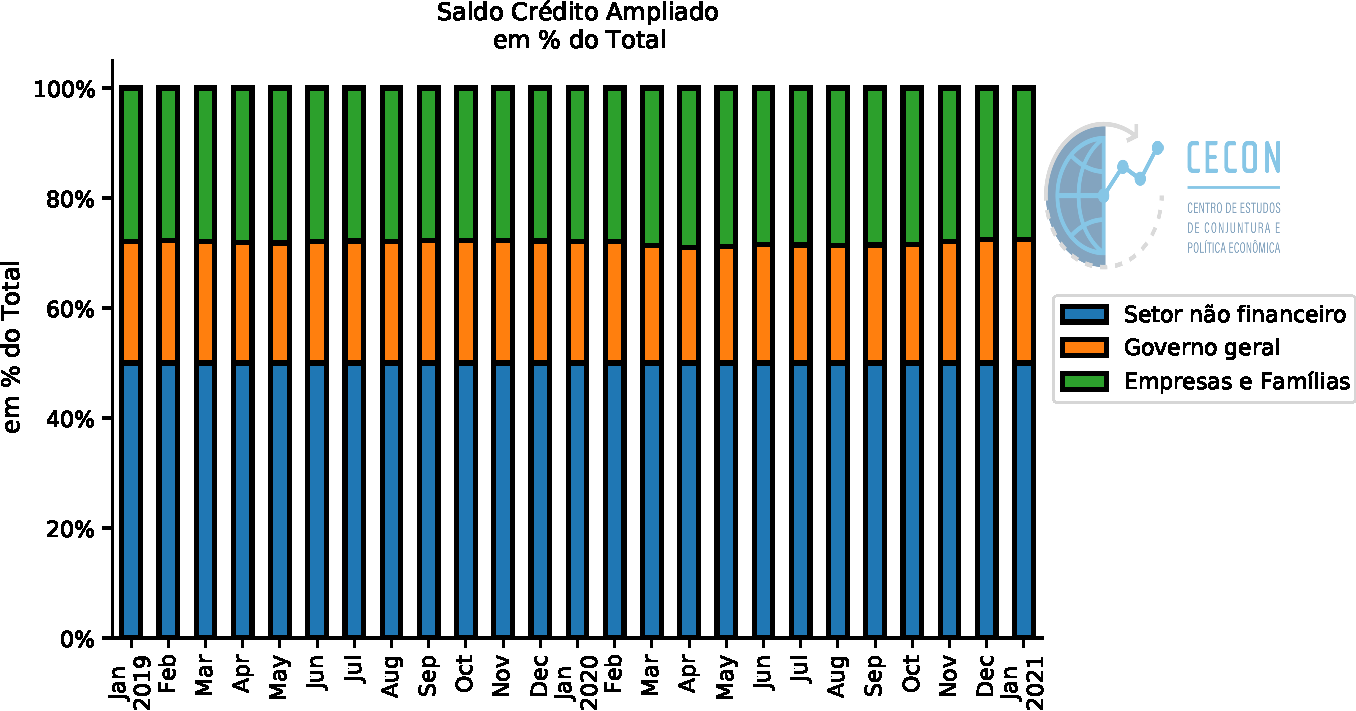
\includegraphics[width=.9\linewidth]{./figs/Credito/SaldoCreditoAmpliado_Total.pdf}
\end{center}

\subsection*{Indicadores de aprovação de crédito}
\label{sec:orgd7c70e8}

\begin{center}
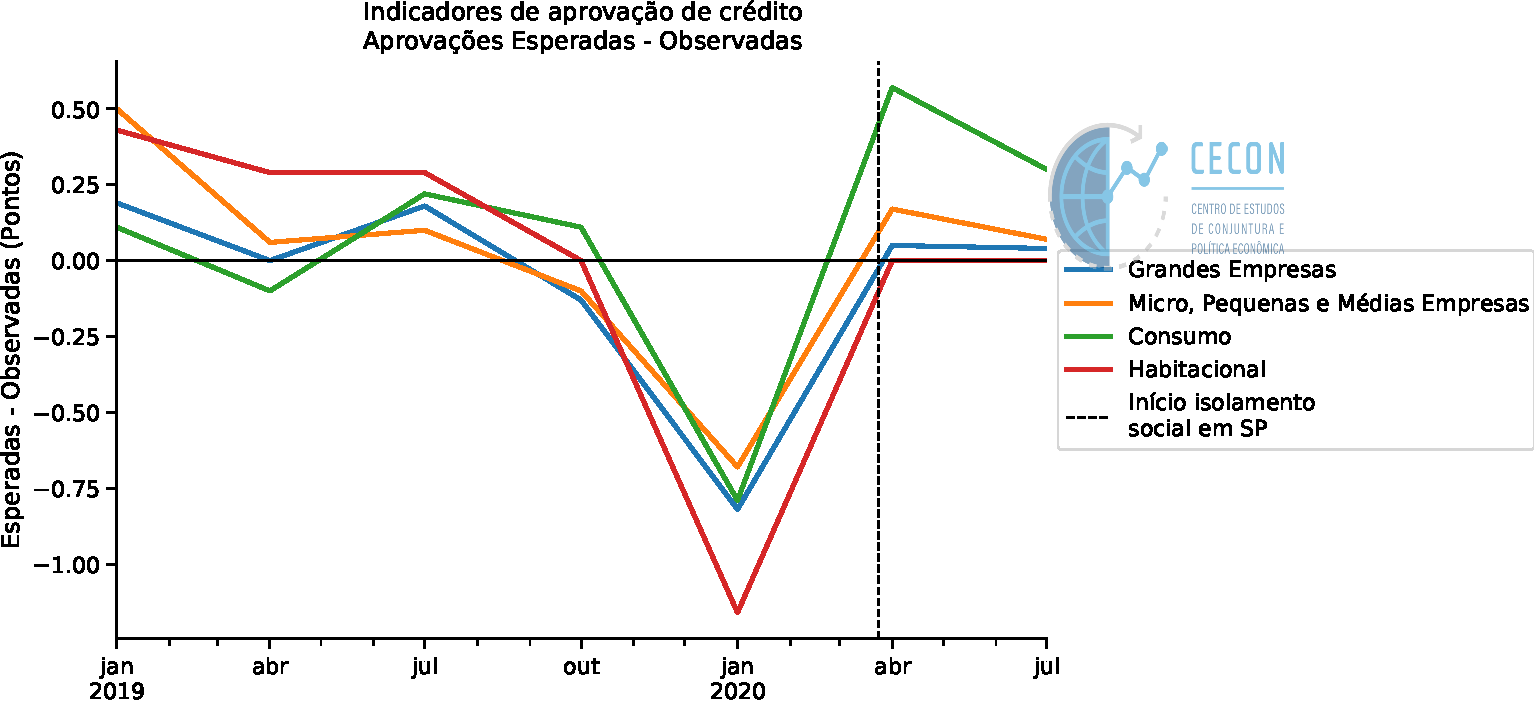
\includegraphics[width=.9\linewidth]{./figs/Credito/PTC.pdf}
\end{center}

\subsection*{Recolhimentos compulsórios de instituições financeiras}
\label{sec:org93a9688}

\begin{center}
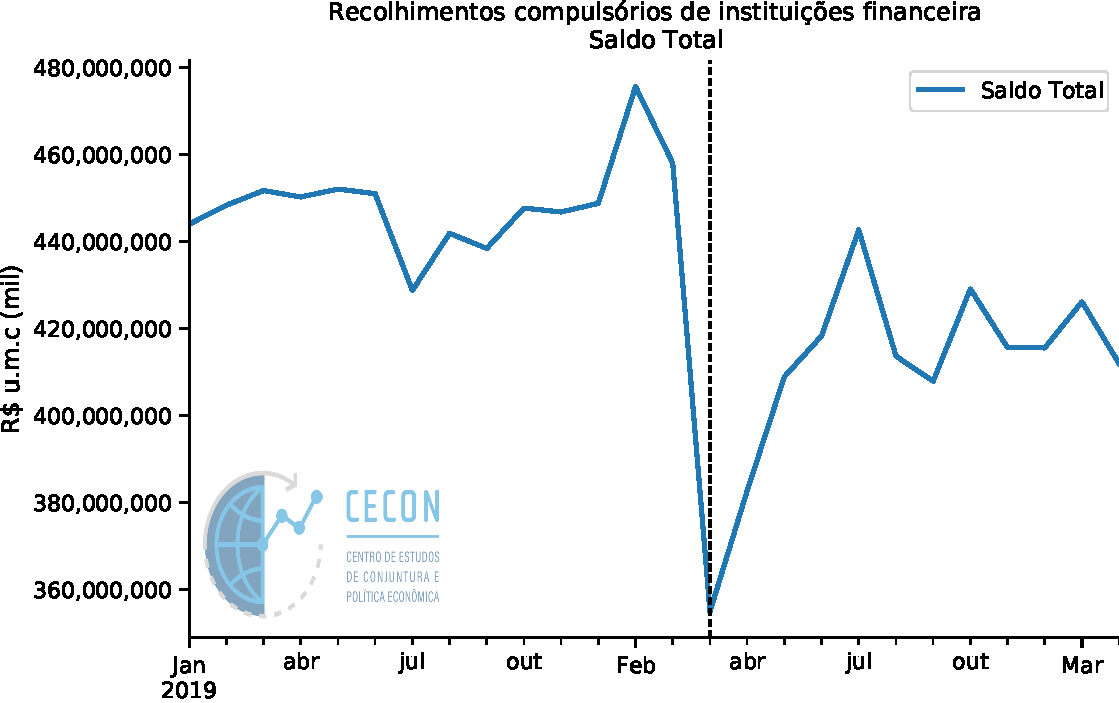
\includegraphics[width=.9\linewidth]{./figs/Credito/Recolhimentos_Total.pdf}
\end{center}

\section*{Índices de atividade setoriais}
\label{sec:org5651375}


\subsection*{Pesquisa Mensal do Comércio (PMC)}
\label{sec:org951f92a}

\begin{center}
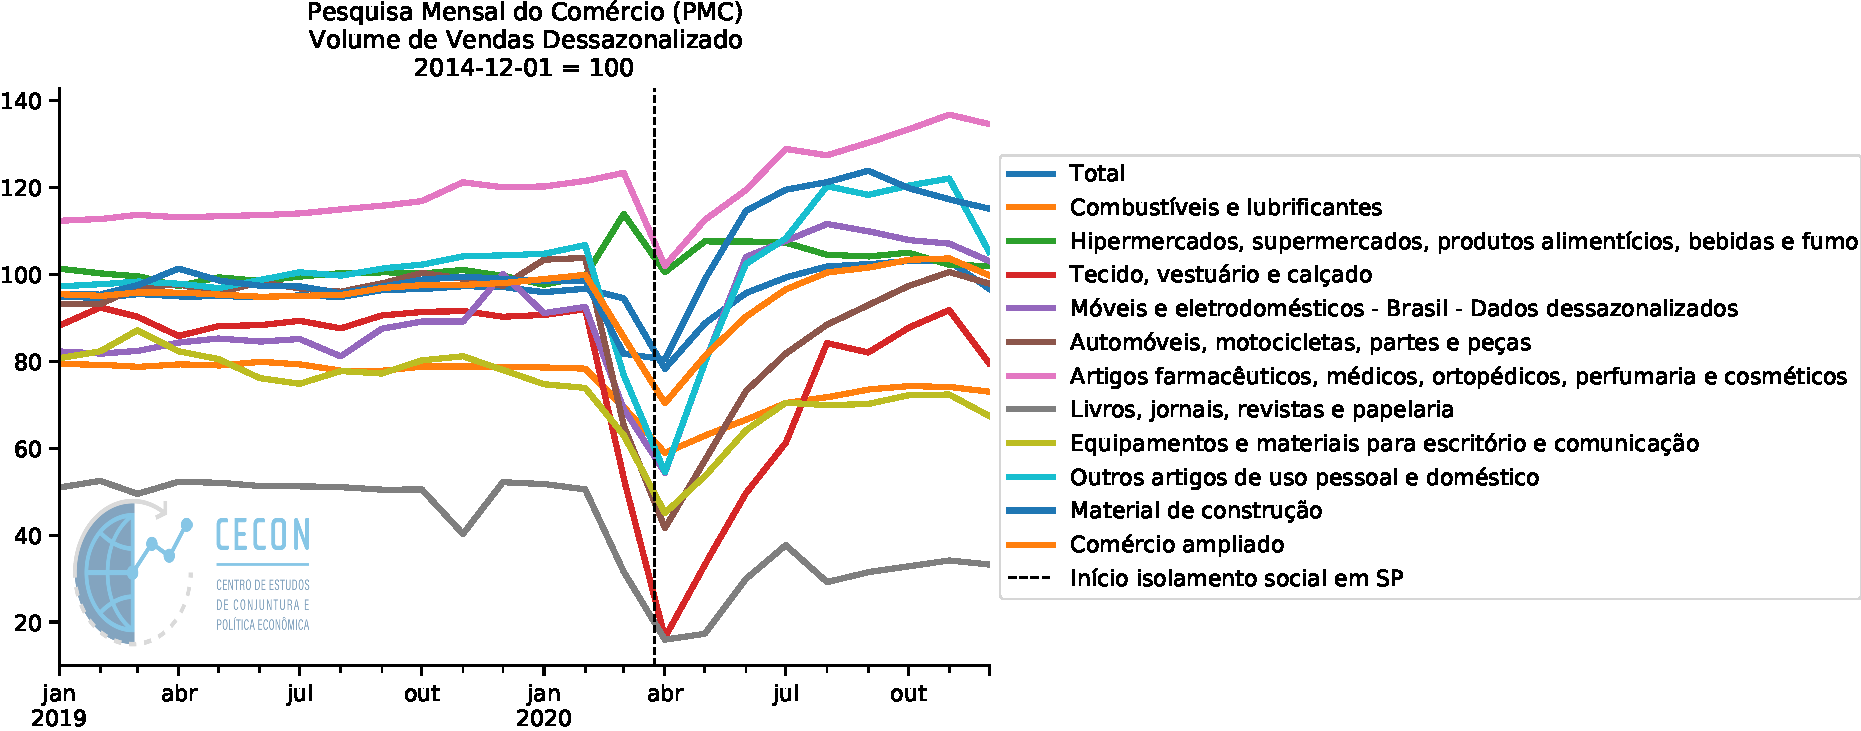
\includegraphics[width=.9\linewidth]{./figs/Setoriais/PMC_IBGE.pdf}
\end{center}


\subsection*{Pesquisa Industrial Mensal (PIM)}
\label{sec:orga7fdf53}

\begin{center}
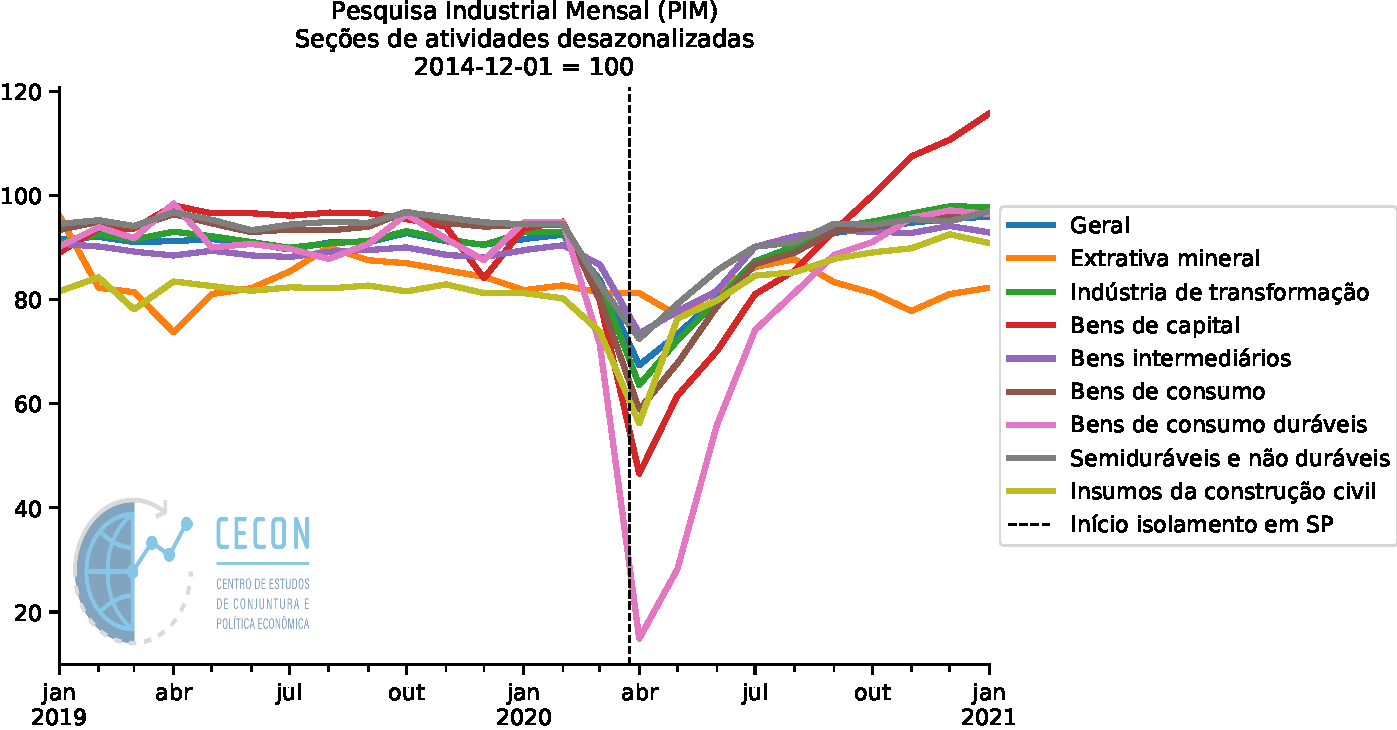
\includegraphics[width=.9\linewidth]{./figs/Setoriais/PIM_IBGE.pdf}
\end{center}


\subsection*{Pesquisa Mensal de Serviços (PMS)}
\label{sec:orgd6e47c4}
\subsubsection*{Receita nominal sem ajuste sazonal}
\label{sec:orgb80d975}
\begin{center}
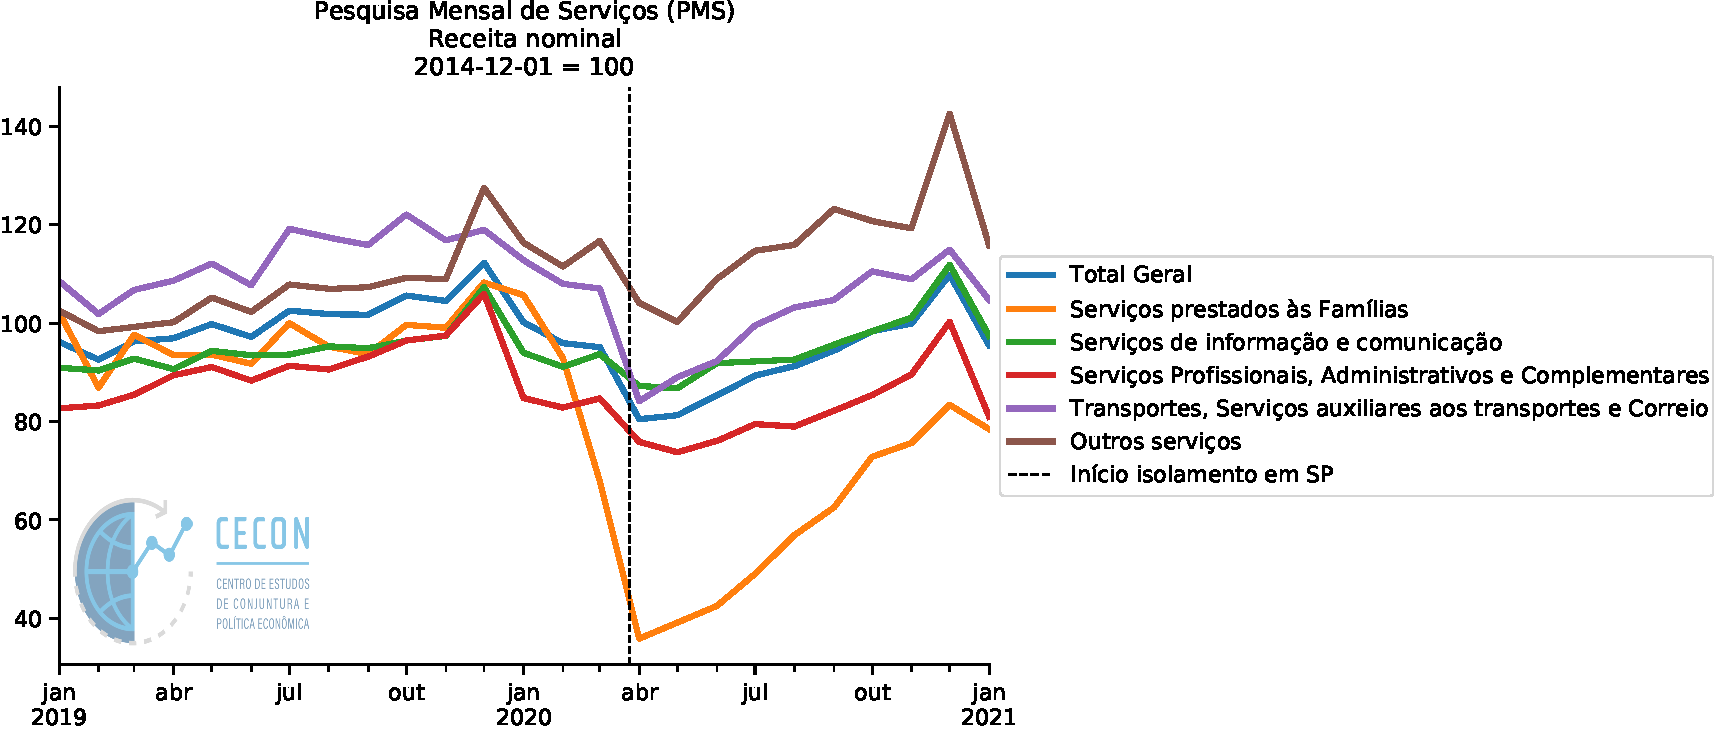
\includegraphics[width=.9\linewidth]{./figs/Setoriais/PMS_IBGE.pdf}
\end{center}

\subsubsection*{Volume com ajuste sazonal}
\label{sec:org9202bab}


\begin{center}
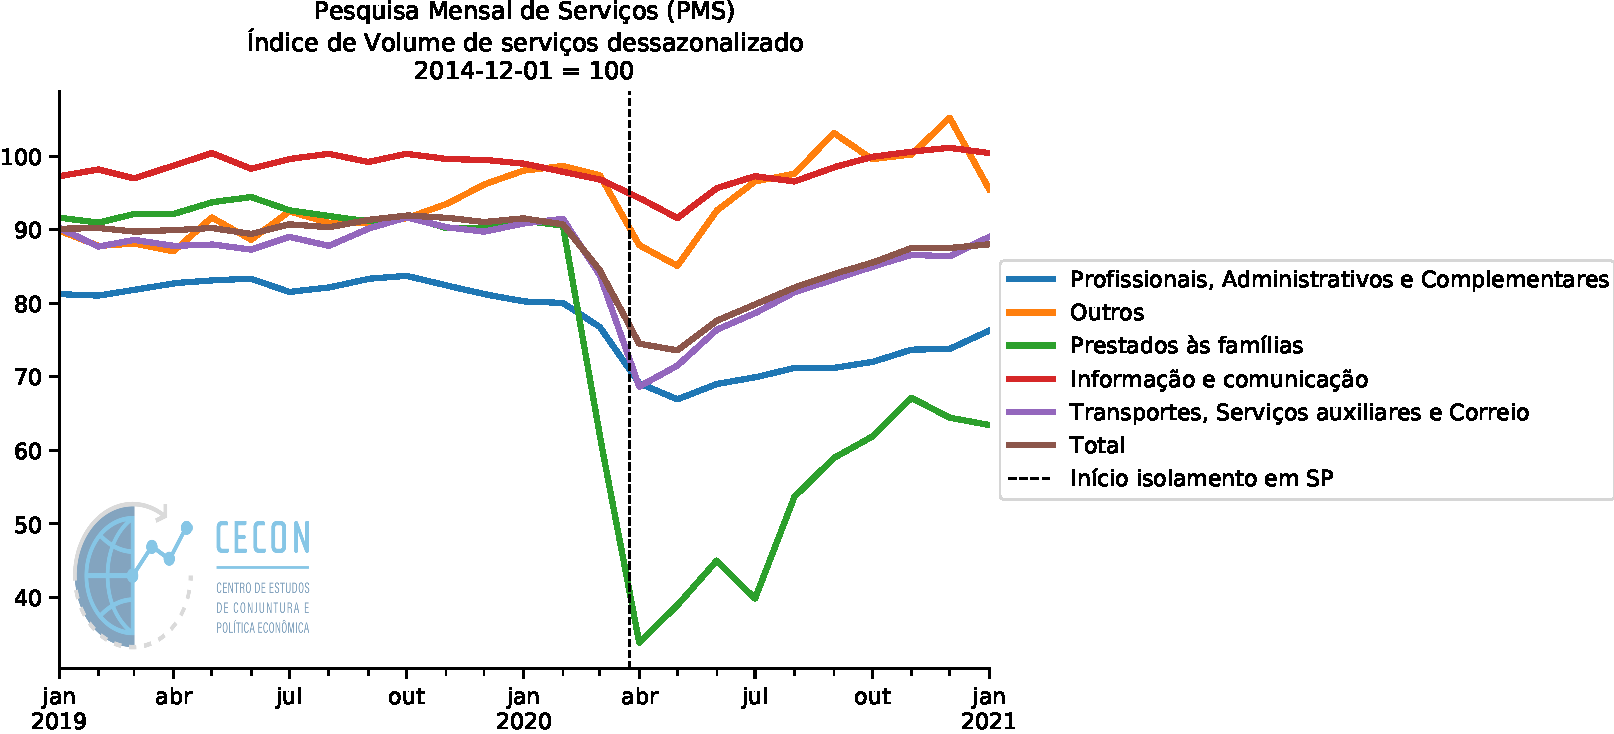
\includegraphics[width=.9\linewidth]{./figs/Setoriais/PMS_vol_dessazonalizada.pdf}
\end{center}

\subsubsection*{Volume com ajuste sazonal (em relação ao mês anterior)}
\label{sec:org5079a18}


\begin{center}
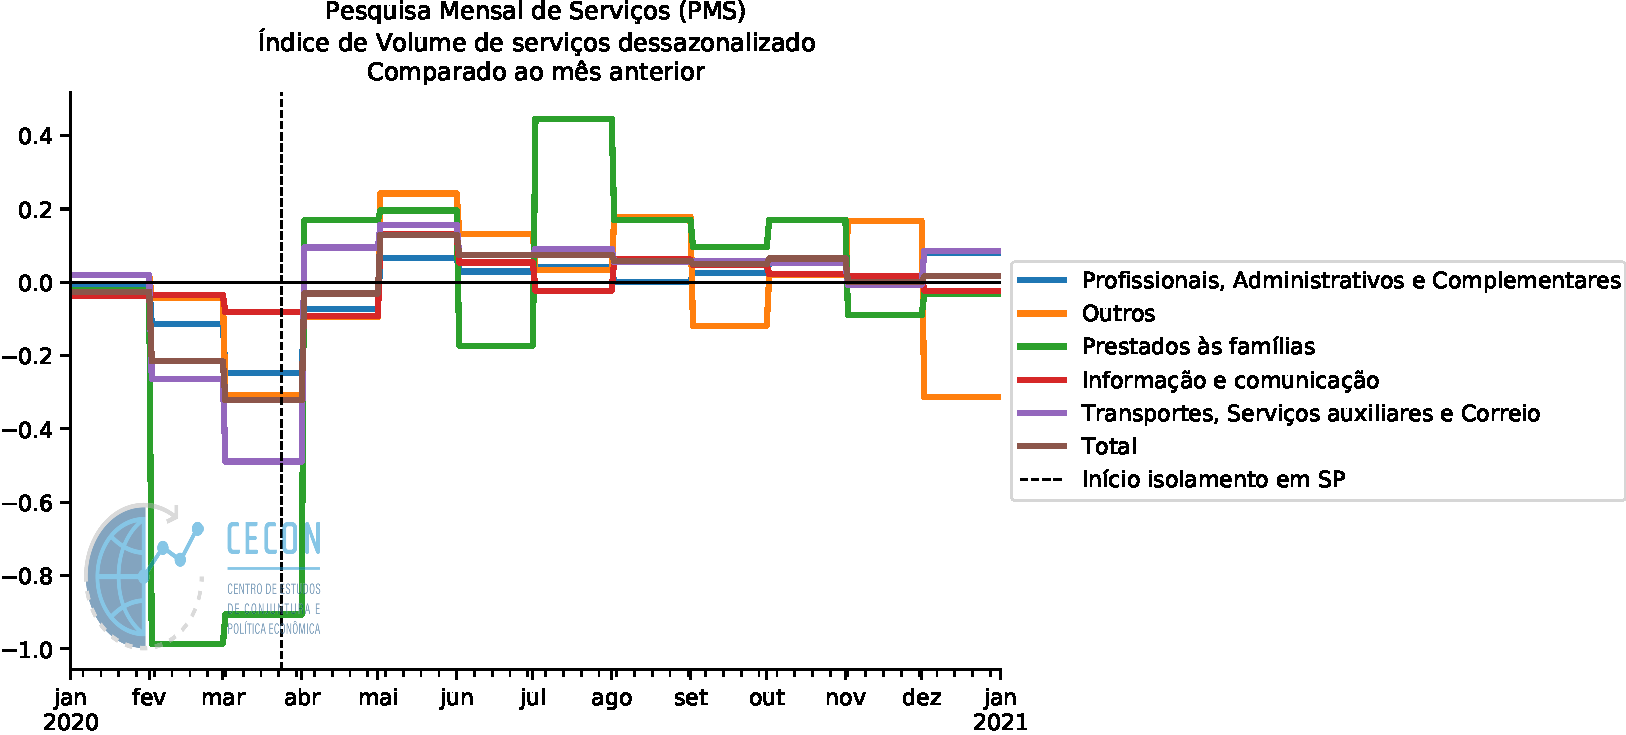
\includegraphics[width=.9\linewidth]{./figs/Setoriais/PMS_vol_dessazonalizada_diff.pdf}
\end{center}

\section*{Emprego}
\label{sec:org249bd60}

\subsection*{Rendimento médio real habitual das pessoas ocupadas}
\label{sec:org8bb81e6}


\begin{center}
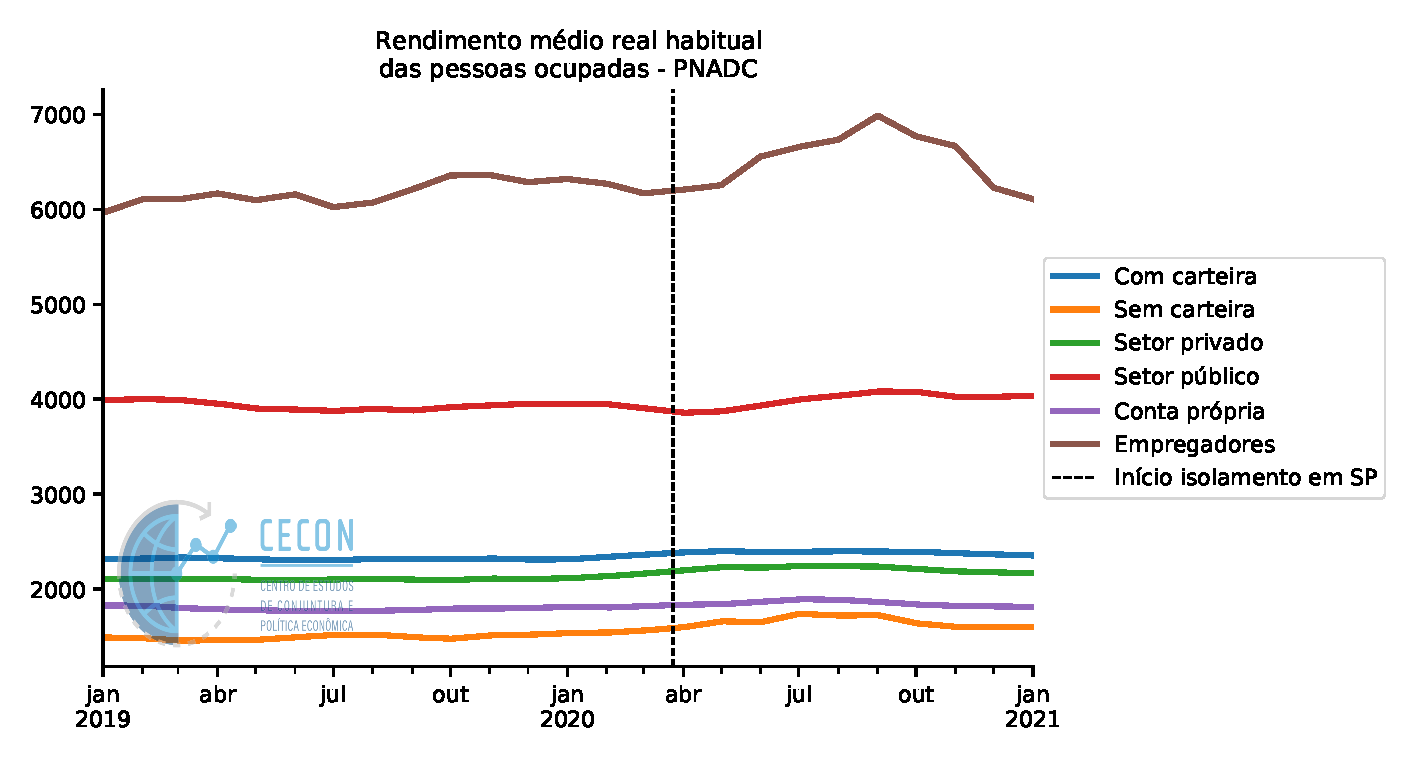
\includegraphics[width=.9\linewidth]{./figs/Emprego/RMHPO.pdf}
\end{center}

\subsection*{Massa de rendimento real efetiva e habitual de todos os trabalhos}
\label{sec:org950156a}

\begin{center}
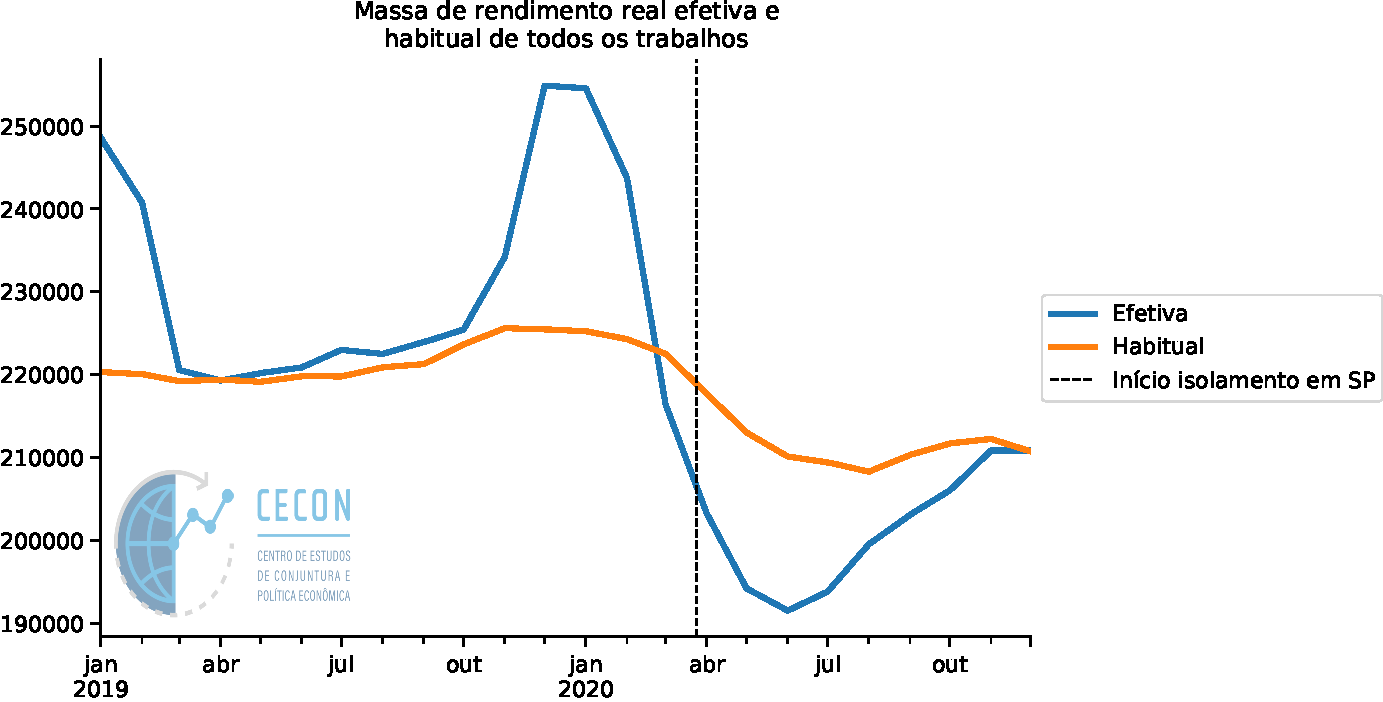
\includegraphics[width=.9\linewidth]{./figs/Emprego/MRR_Efetiva_Habitual.pdf}
\end{center}

\subsection*{Massa Salarial Ampliada Disponível - PNADC}
\label{sec:org005c644}

\begin{center}
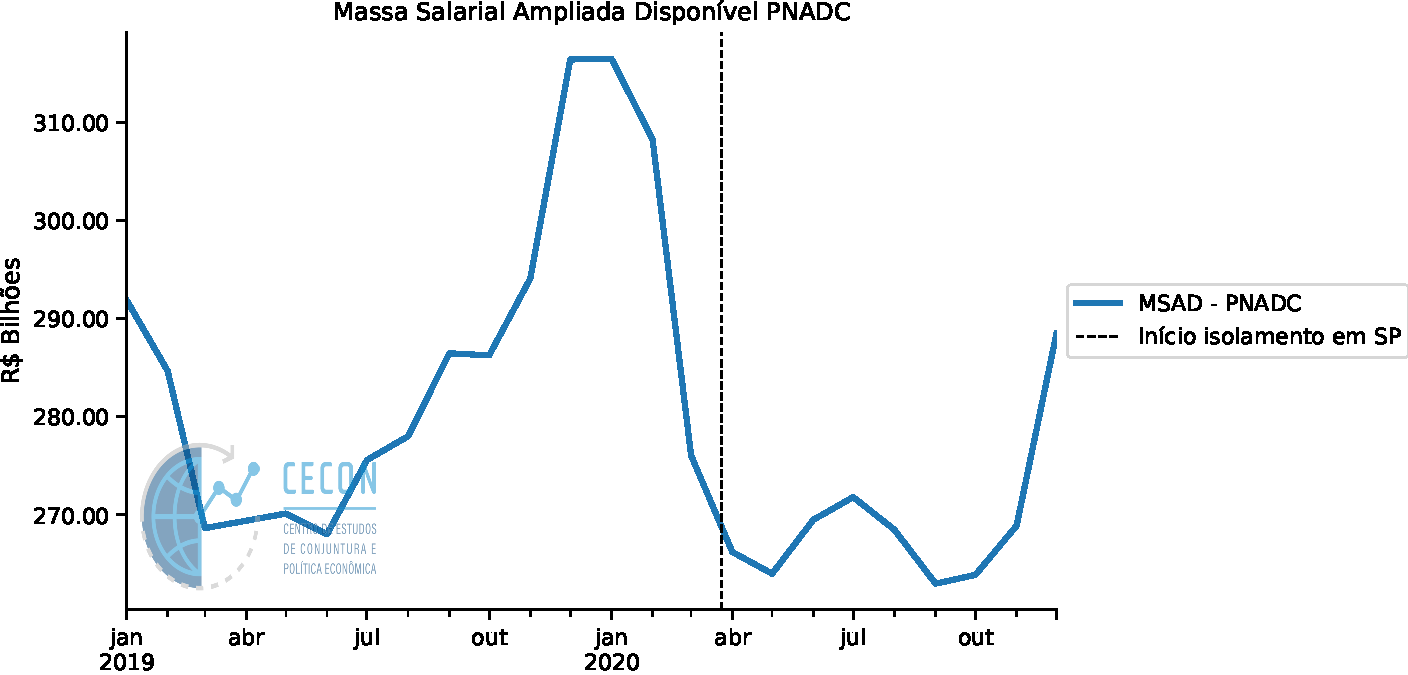
\includegraphics[width=.9\linewidth]{./figs/Emprego/MSAD.pdf}
\end{center}

\subsection*{Rendimento habitual médio por atividade}
\label{sec:org542f1ff}

\subsection*{Número de horas trabalhadas - indústria de transformação}
\label{sec:org5d2cb27}

\begin{center}
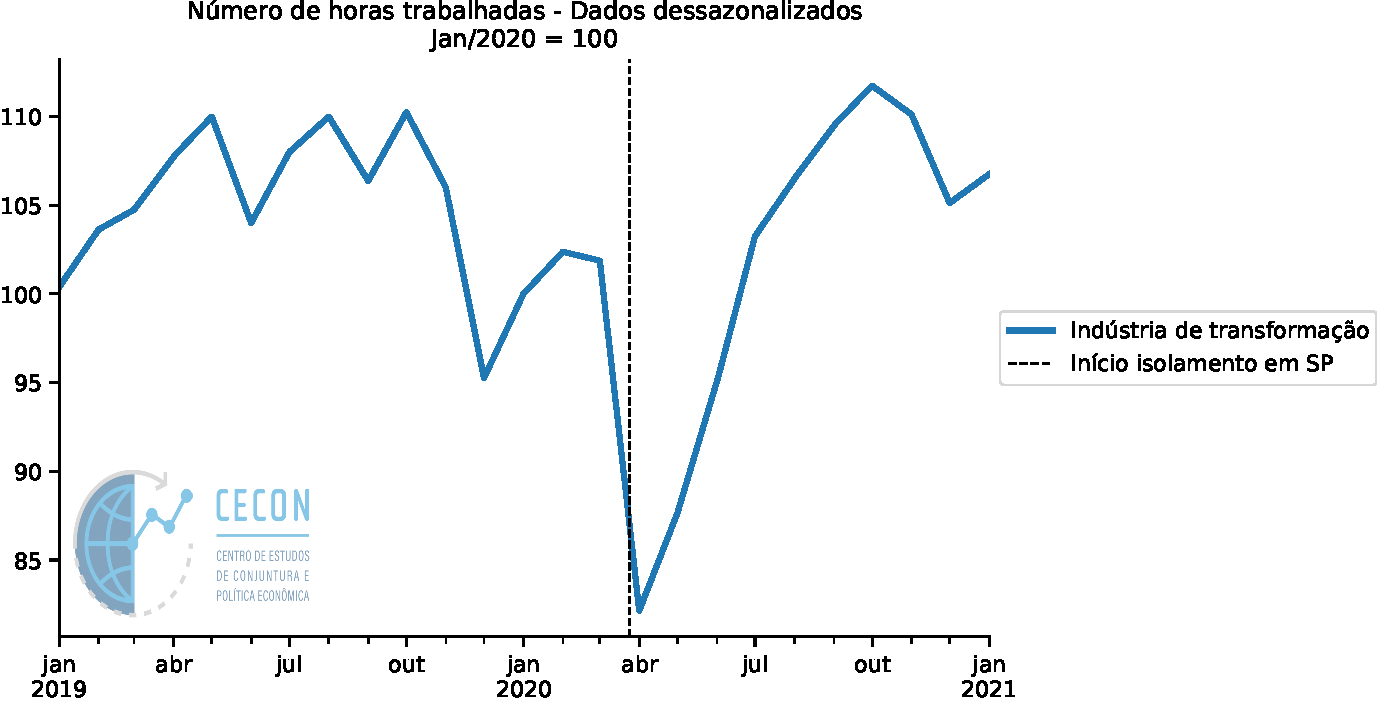
\includegraphics[width=.9\linewidth]{./figs/Emprego/Horas_Transformacao.pdf}
\end{center}

\subsection*{Novo CAGED  - Por atividade (dados dessazonalizados)}
\label{sec:org3996ac5}

\begin{center}
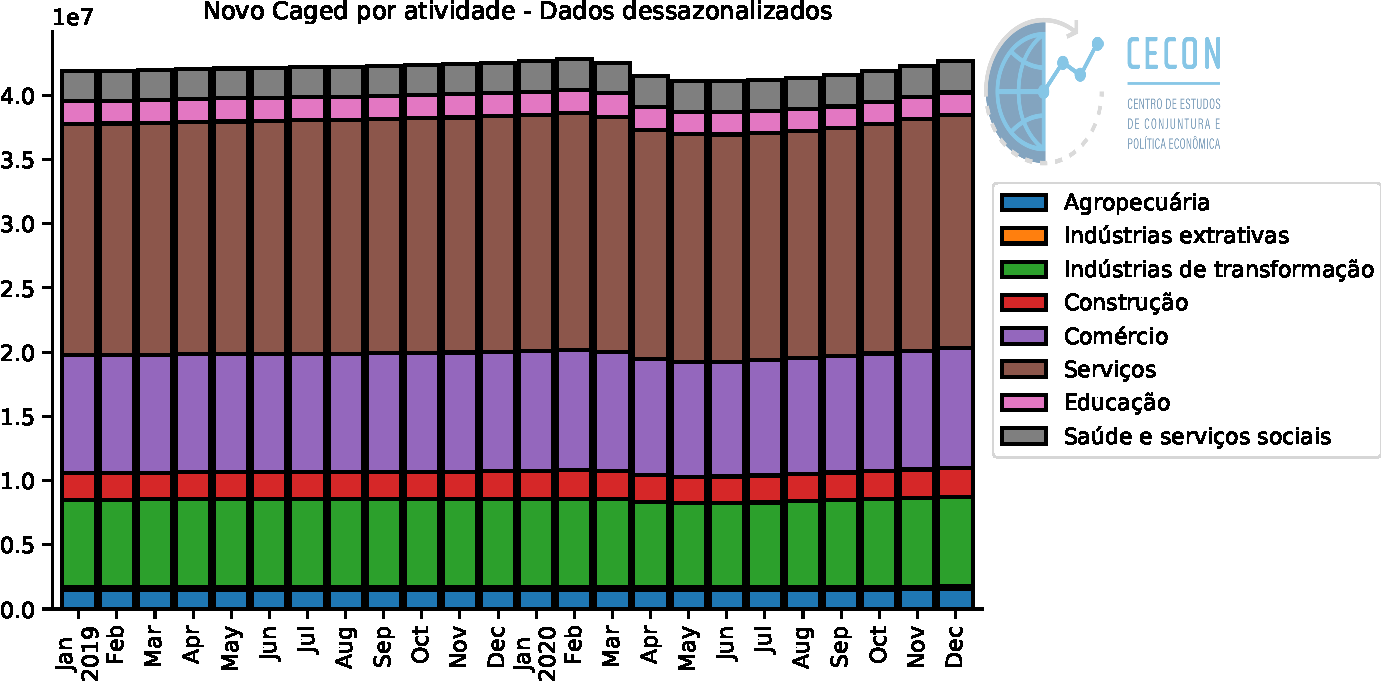
\includegraphics[width=.9\linewidth]{./figs/Emprego/NovoCaged_Atividade.pdf}
\end{center}



\subsection*{Taxa de desocupação}
\label{sec:org838641f}

\begin{center}
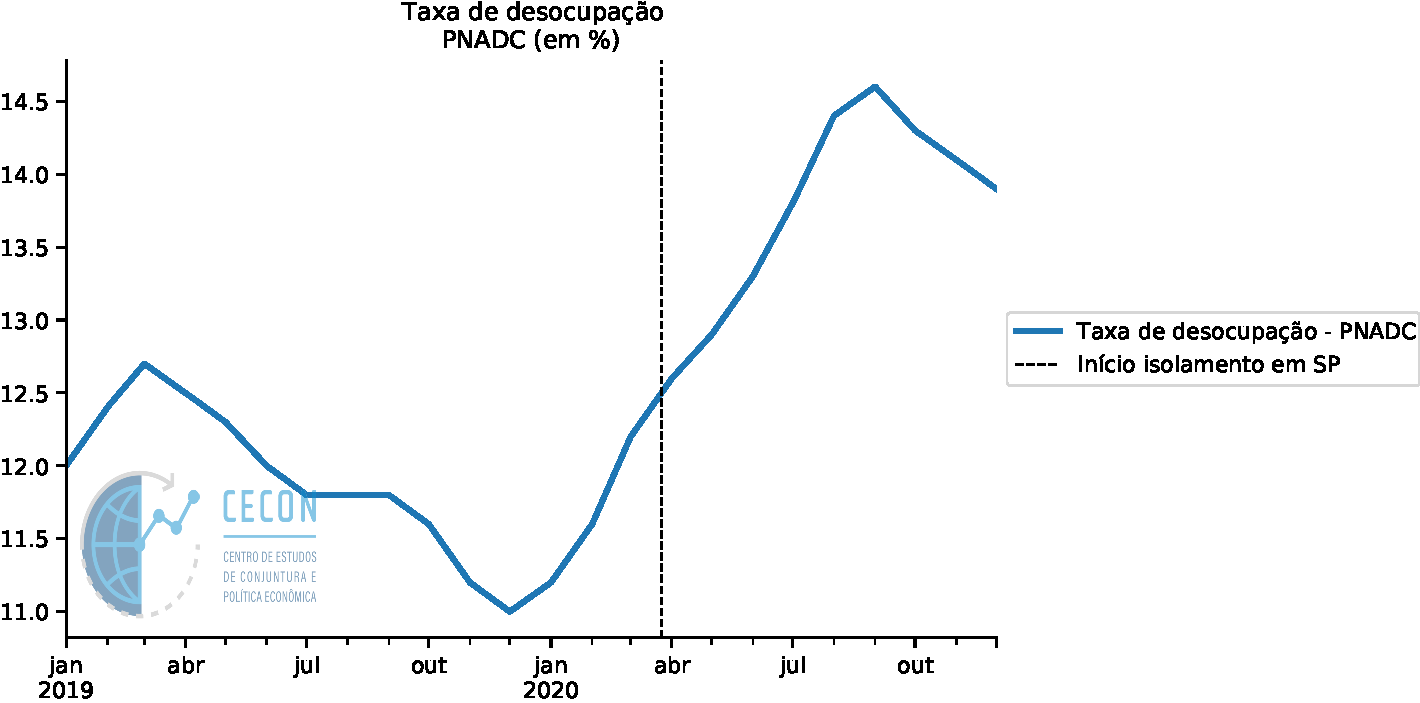
\includegraphics[width=.9\linewidth]{./figs/Emprego/TaxaDesocupacao.pdf}
\end{center}

\section*{PNAD-COVID}
\label{sec:org5e27dc1}
\subsection*{R trial}
\label{sec:orgee05f25}
\subsection*{Home office - Por sexo e cor}
\label{sec:org7558892}




\begin{center}
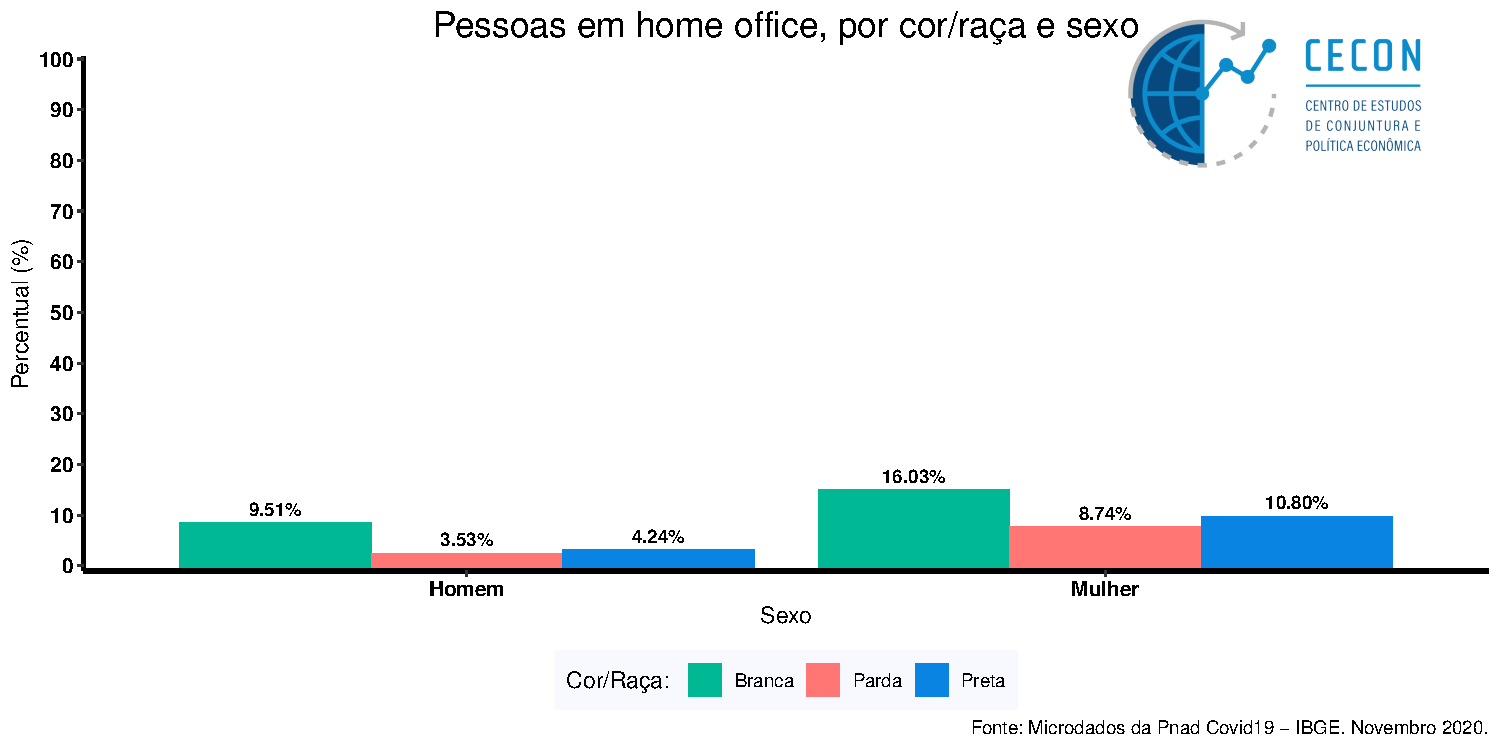
\includegraphics[width=.9\linewidth]{./figs/PNAD_COVID/home_sexo_cor.pdf}
\end{center}

\subsection*{Home office - Por Cor e Escolaridade}
\label{sec:org8915d79}
\begin{center}
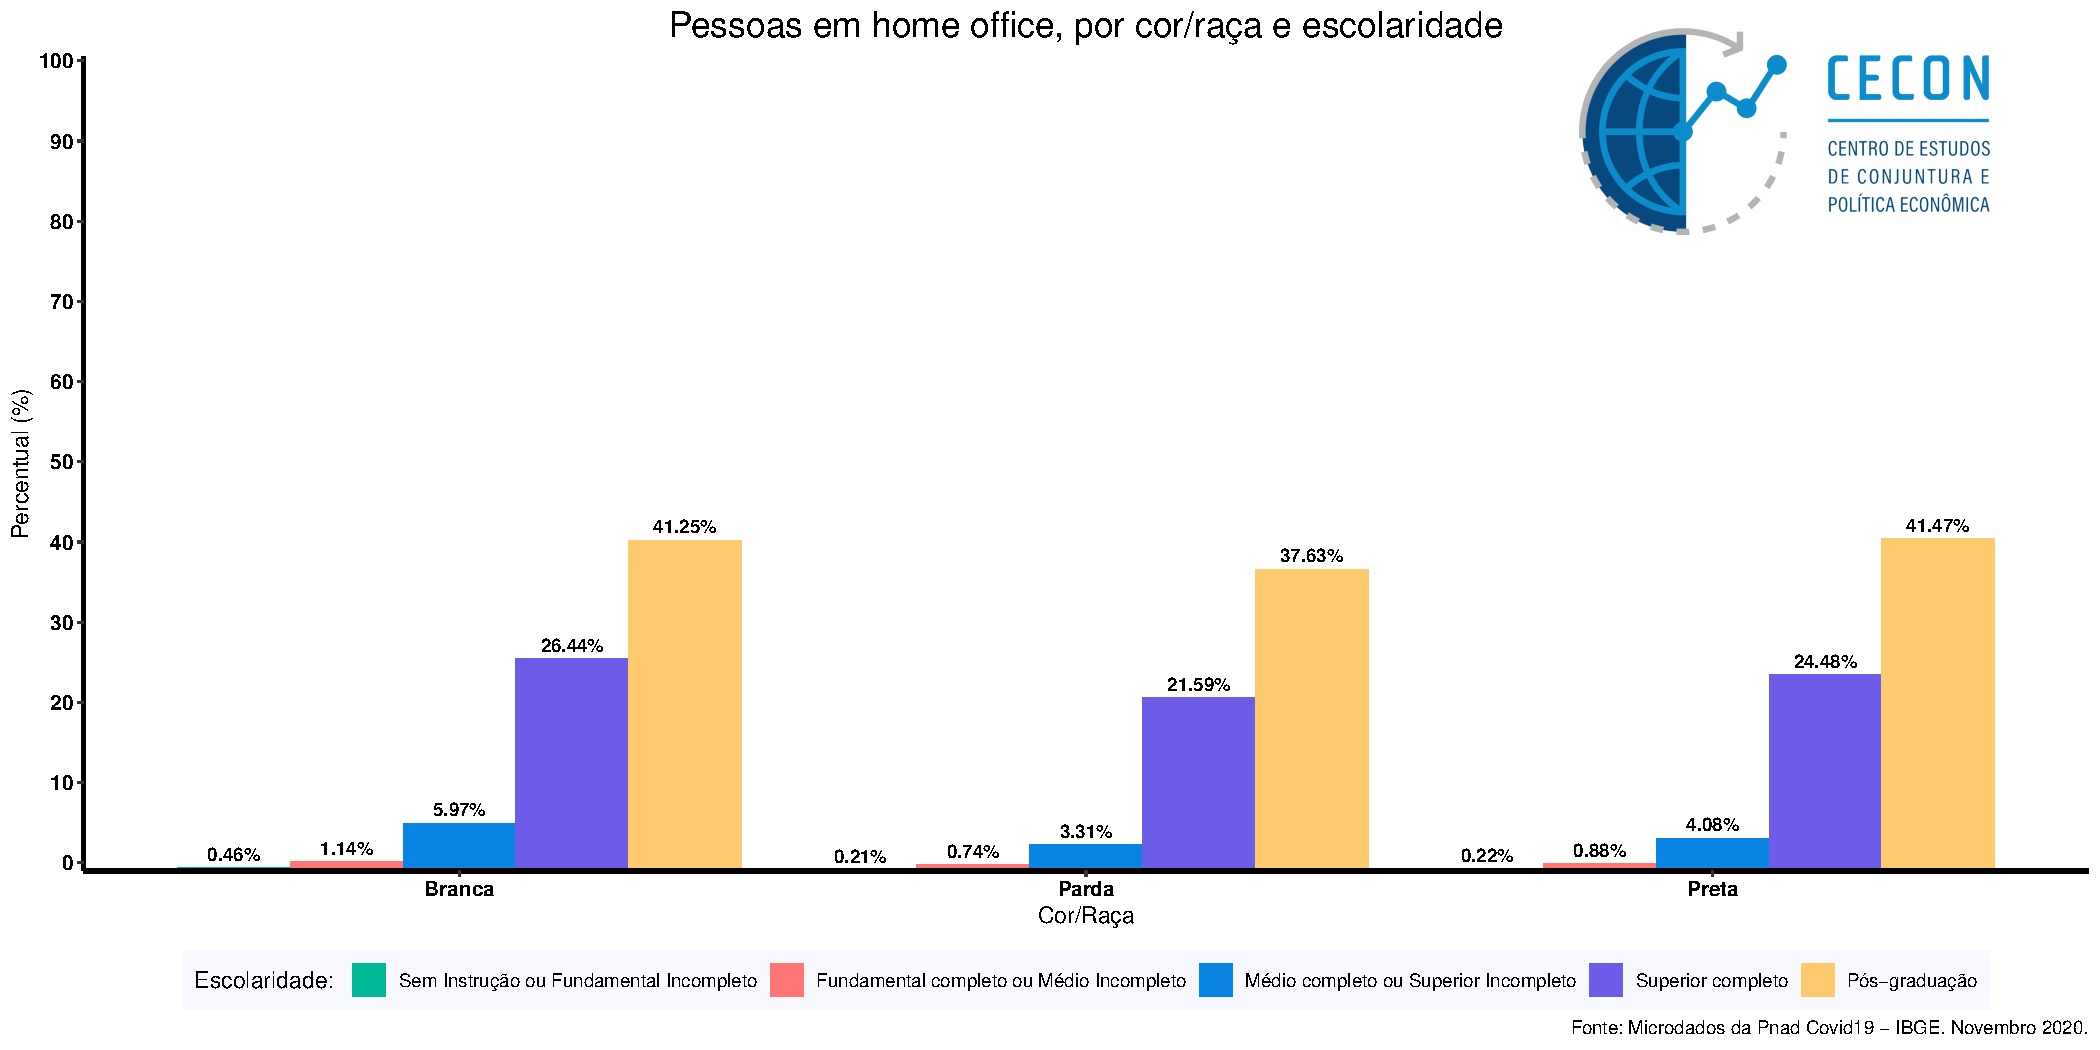
\includegraphics[width=.9\linewidth]{./figs/PNAD_COVID/home_edu_cor.pdf}
\end{center}
\subsection*{Home office - Por Cor e Idade}
\label{sec:org9262d3d}
\begin{center}
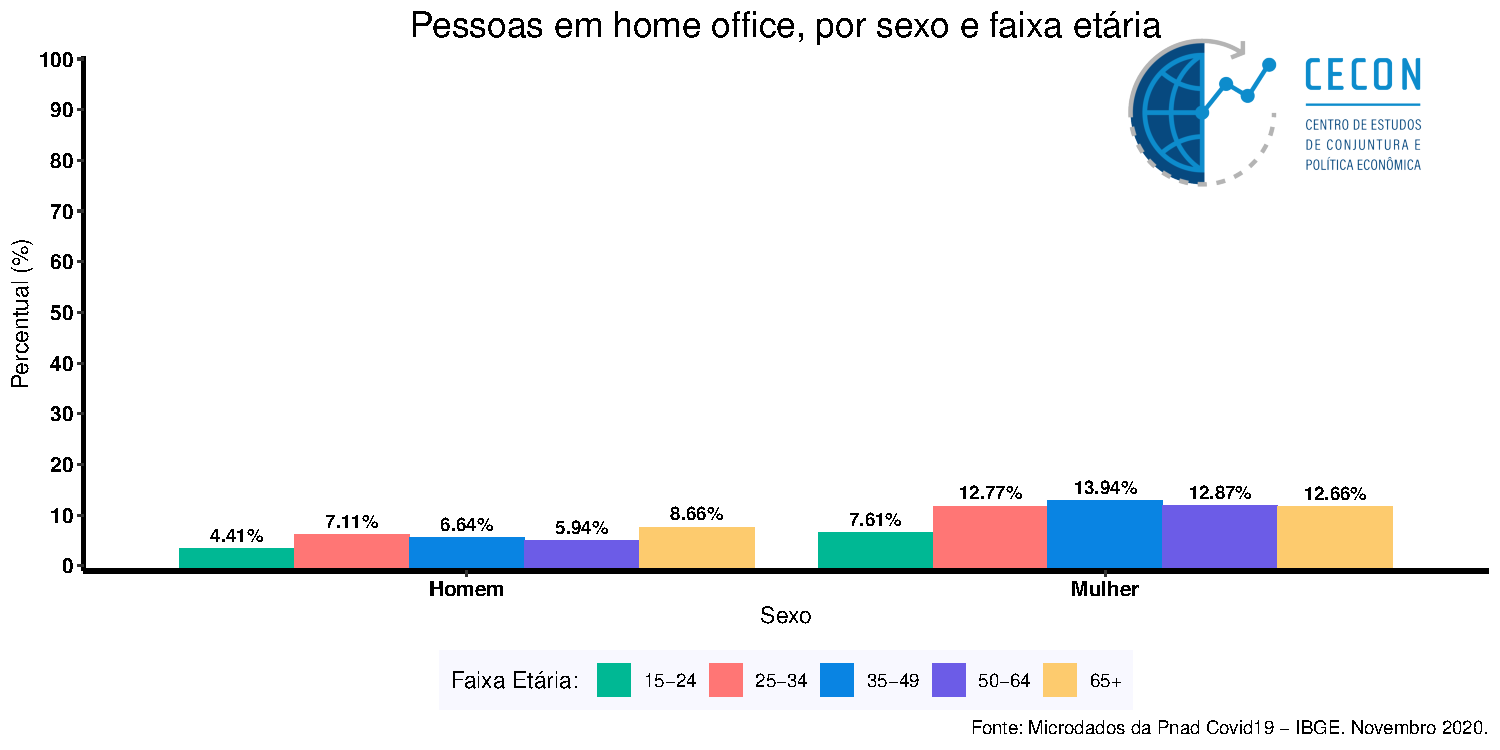
\includegraphics[width=.9\linewidth]{./figs/PNAD_COVID/home_sexo_idade.pdf}
\end{center}

\subsection*{Home office - Por Trabalho}
\label{sec:org69feb9a}
\begin{center}
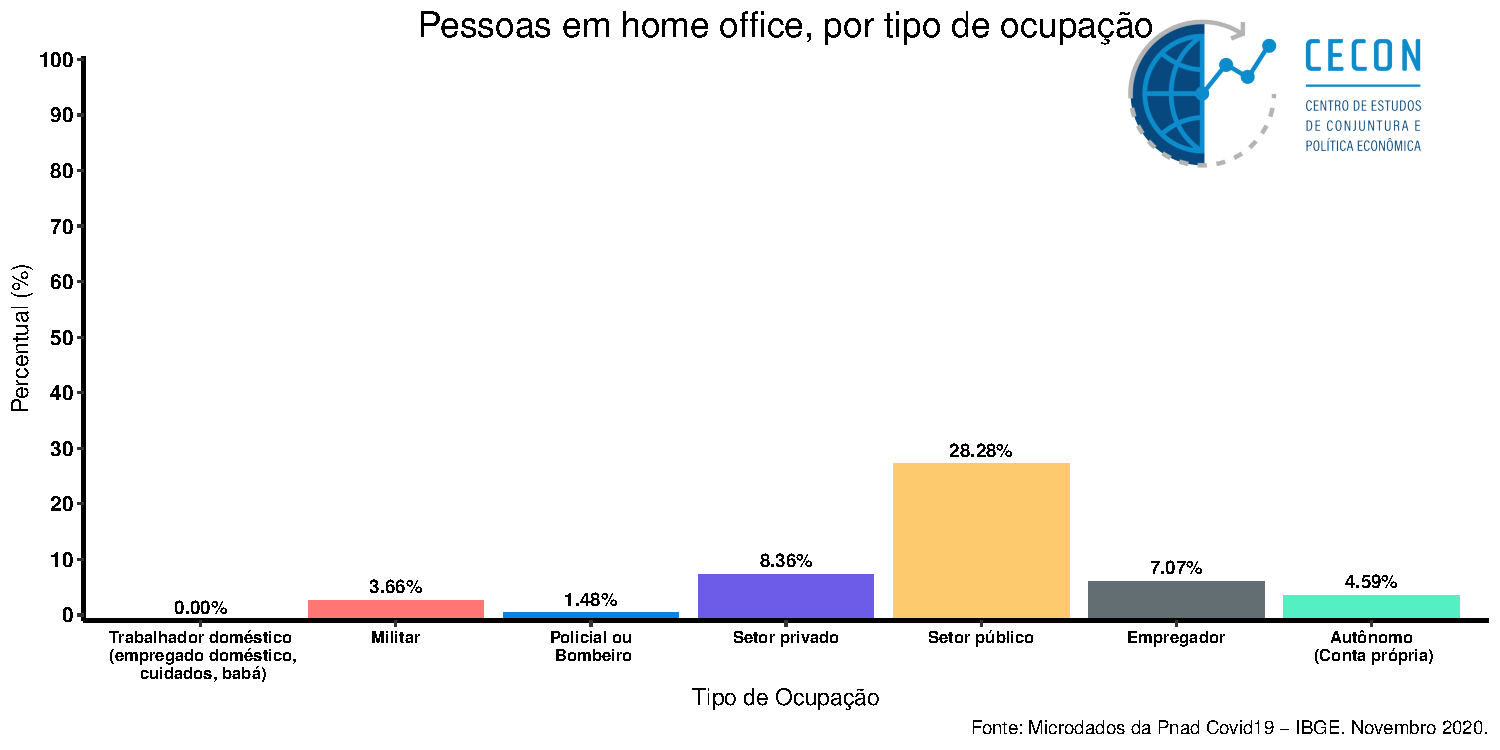
\includegraphics[width=.9\linewidth]{./figs/PNAD_COVID/home_emprego.pdf}
\end{center}

\subsection*{Home office - Por faixa salarial e cor}
\label{sec:org39eb121}
\begin{center}
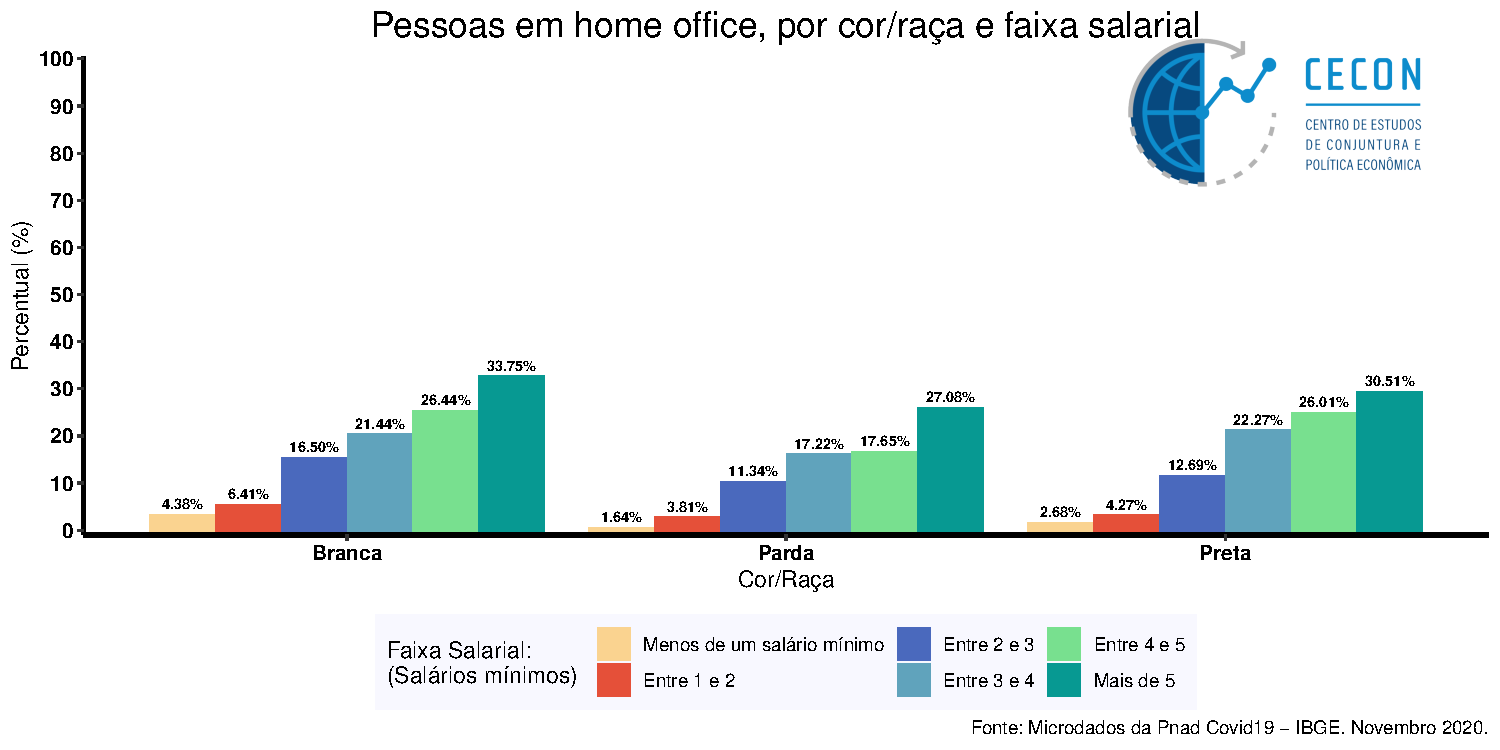
\includegraphics[width=.9\linewidth]{./figs/PNAD_COVID/home_renda.pdf}
\end{center}
\subsection*{Auxilio - Faixa Salarial}
\label{sec:orgf9f1894}
\begin{center}
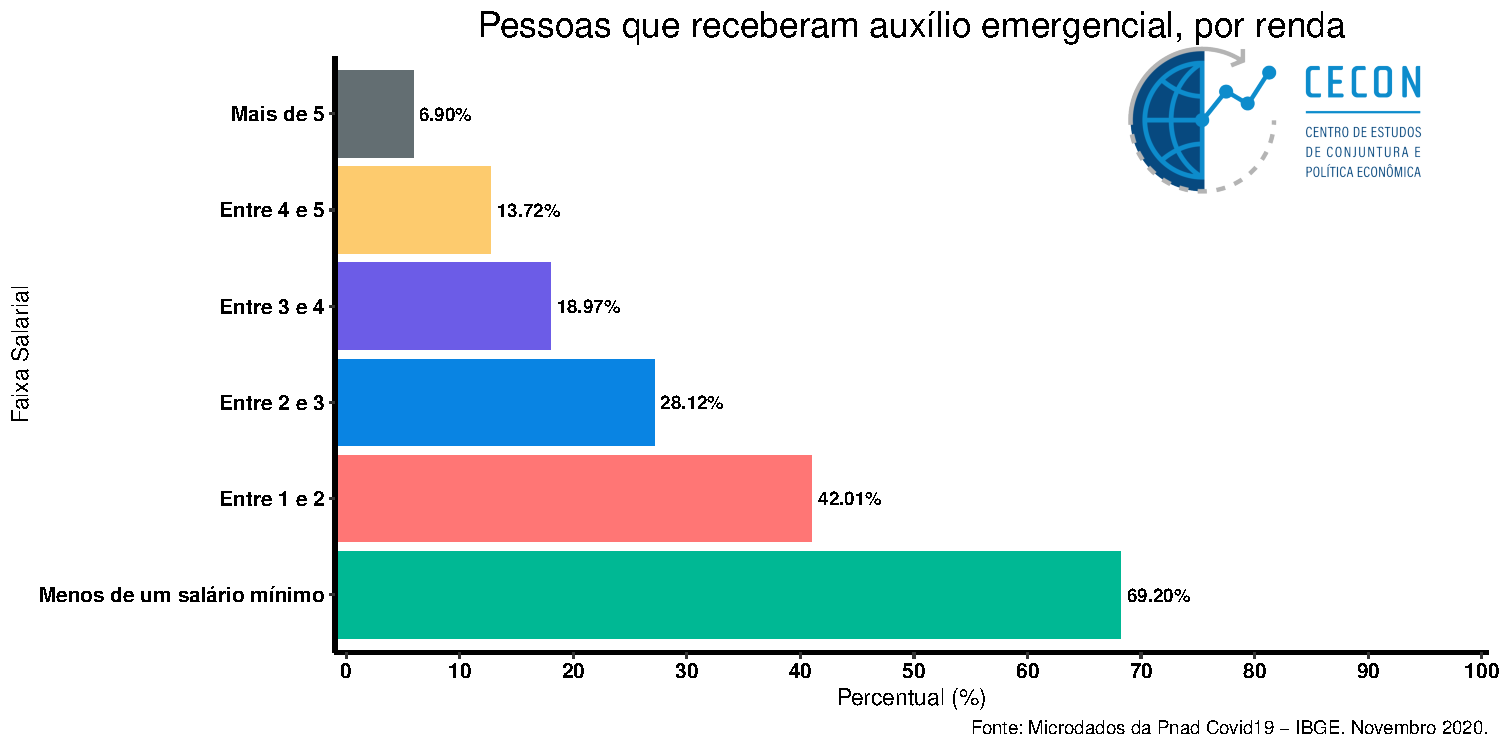
\includegraphics[width=.9\linewidth]{./figs/PNAD_COVID/auxilio_renda.pdf}
\end{center}
\subsection*{Auxilio - Por tipo do domicilio}
\label{sec:orgc6848b7}
\begin{center}
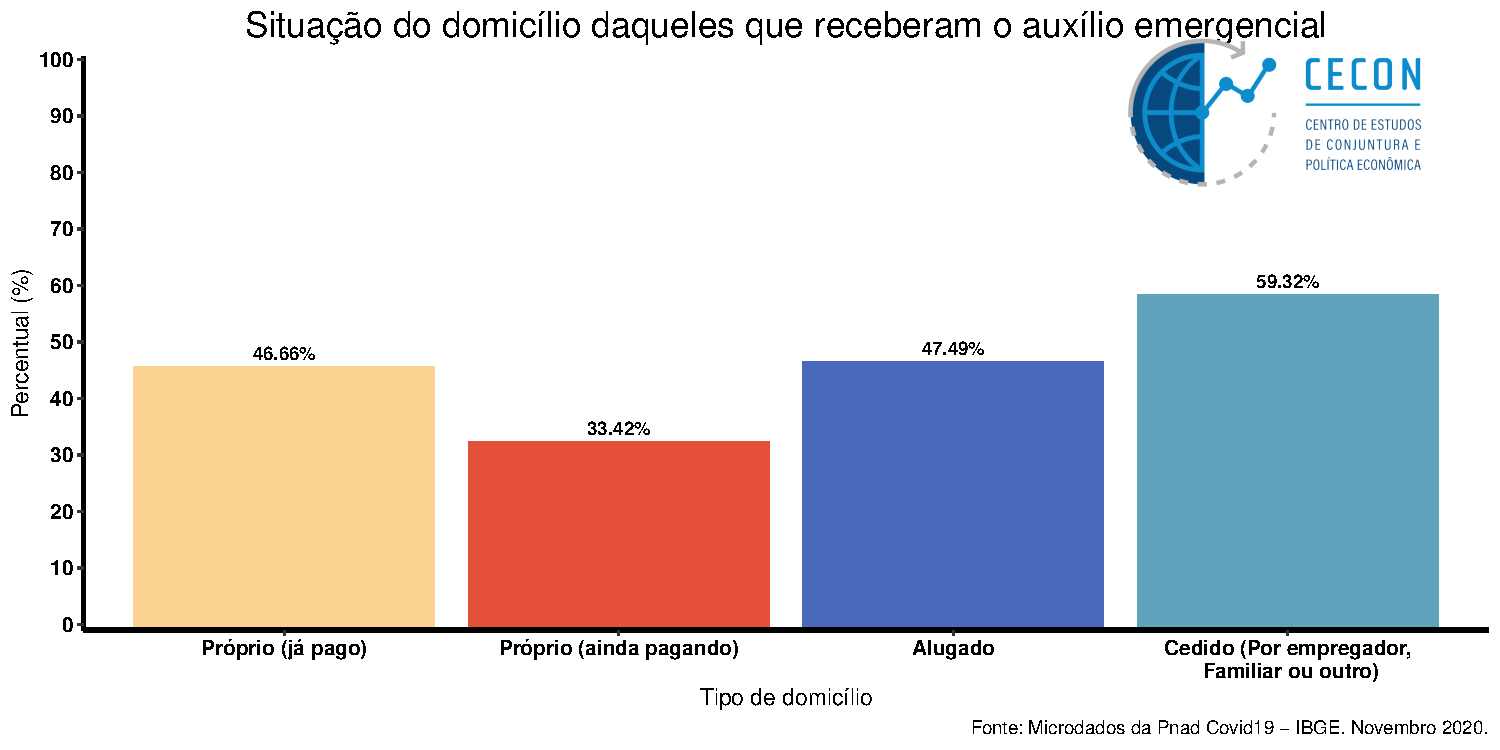
\includegraphics[width=.9\linewidth]{./figs/PNAD_COVID/auxilio_domicilio.pdf}
\end{center}
\subsection*{Auxilio - Sexo e Cor}
\label{sec:org0dcd808}
\begin{center}
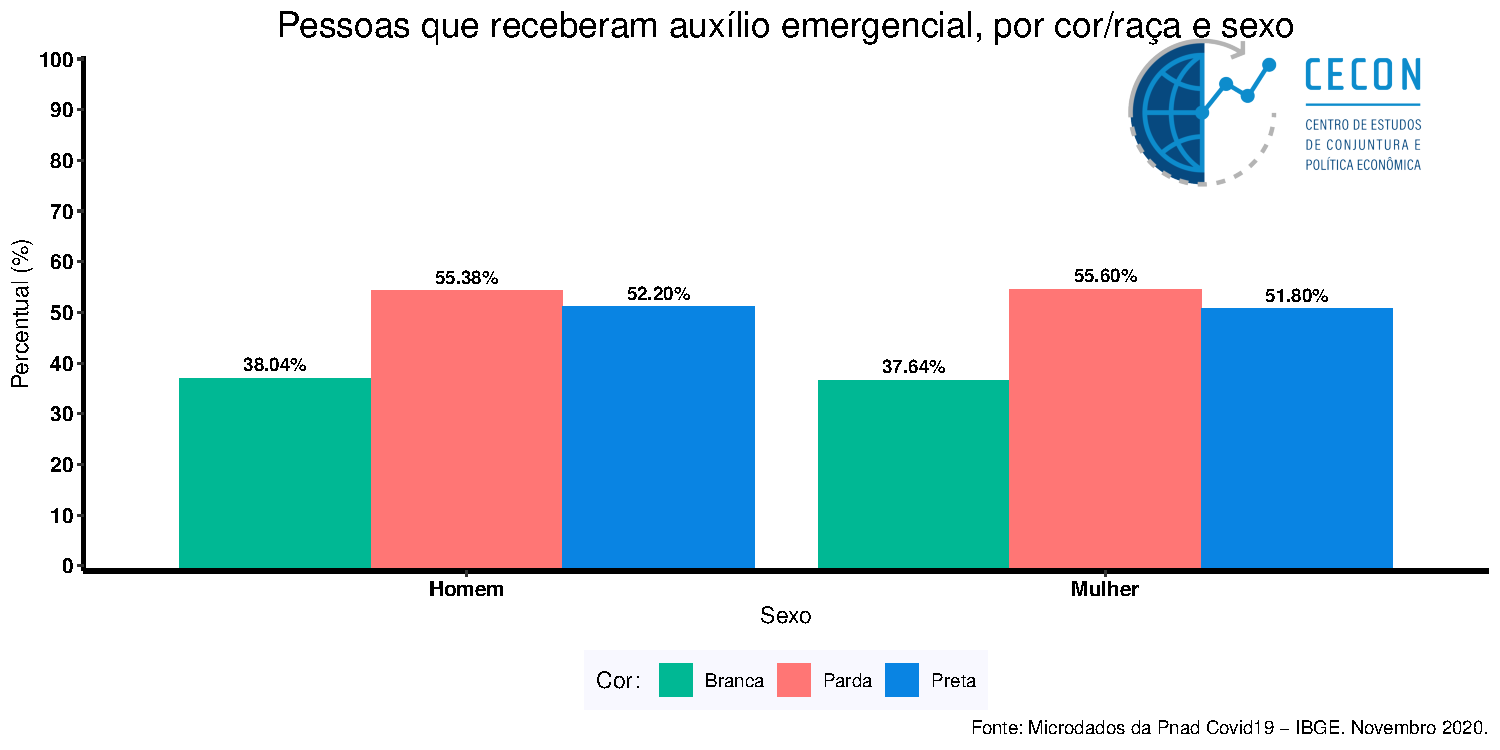
\includegraphics[width=.9\linewidth]{./figs/PNAD_COVID/auxilio_cor_sexo.pdf}
\end{center}


\section*{IMF Fiscal Monitor}
\label{sec:org57e1cdc}
\subsection*{Medidas fiscais em \% do PIB}
\label{sec:orga4b325a}

\begin{center}
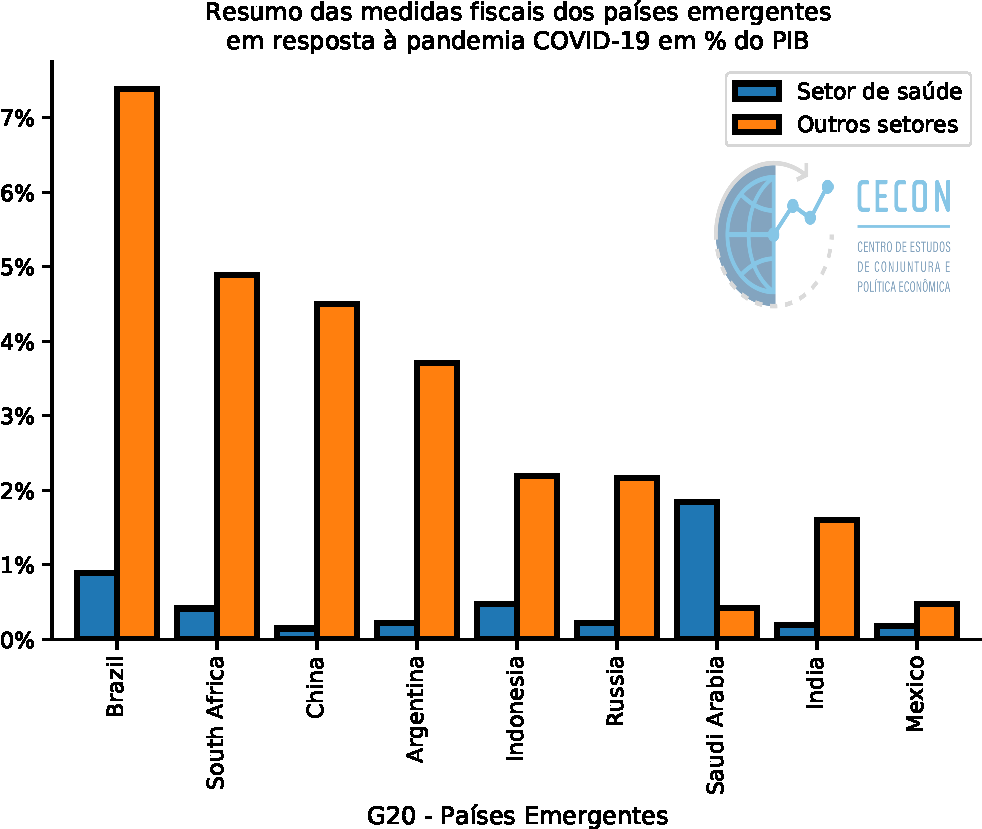
\includegraphics[width=.9\linewidth]{./figs/IMF/FiscalMonitor_Covid.pdf}
\end{center}

\subsection*{Medidas fiscais em \% do PIB: Setor de saúde/Outros setores}
\label{sec:org55c3d2a}

\begin{center}
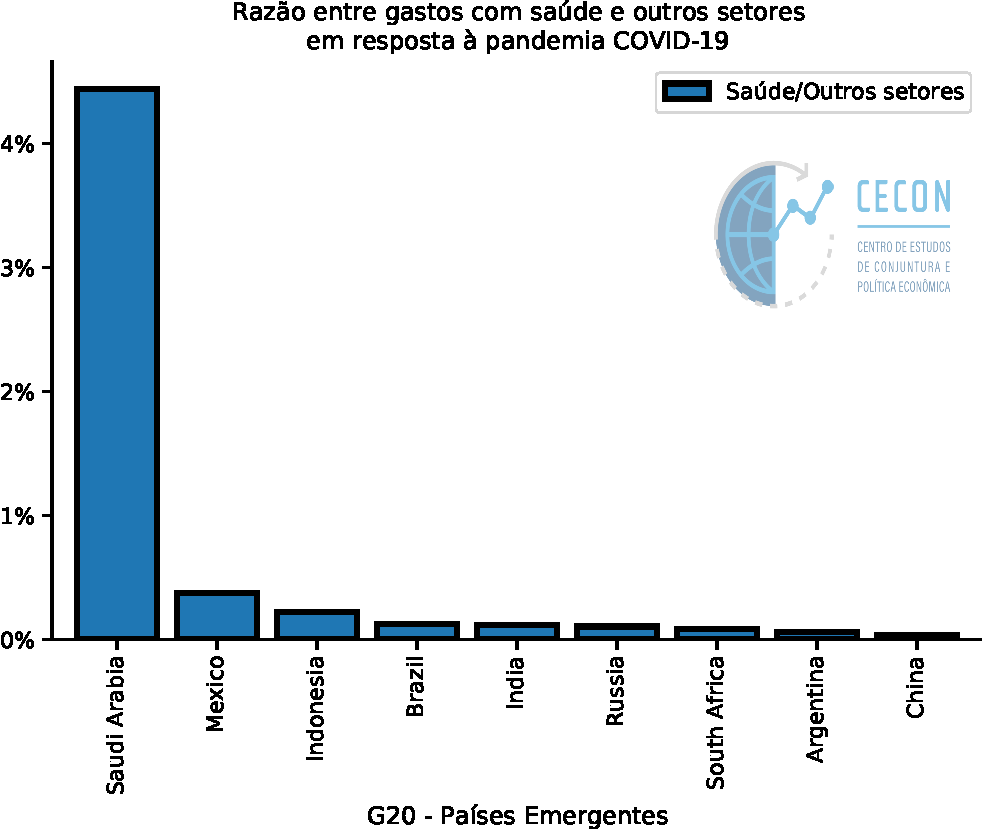
\includegraphics[width=.9\linewidth]{./figs/IMF/FiscalMonitor_Covid_ratio.pdf}
\end{center}

\subsection*{Medidas fiscais em \% do PIB: Setor de saúde/Total}
\label{sec:org3509d44}

\begin{center}
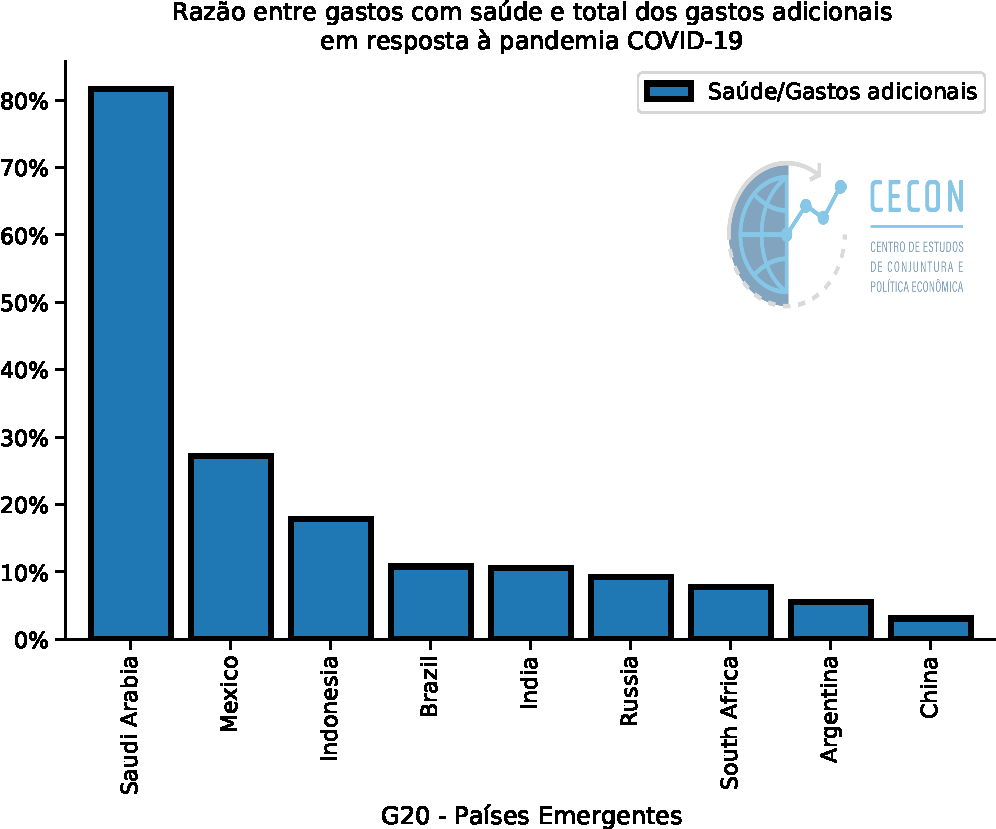
\includegraphics[width=.9\linewidth]{./figs/IMF/FiscalMonitor_Covid_total.pdf}
\end{center}

\section*{World Economic outlook}
\label{sec:org99cb48b}


\subsection*{GDP vs Lockdown}
\label{sec:orgd0bd47c}
\begin{table}[htbp]
\caption{\label{IMF_fig_1}GDP Forecast Errors in 2020:H1 and Lockdown Stringency}
\centering
\begin{tabular}{lll}
\hline
Country & GDP Forecast Error & Lockdown Stringency\\
\hline
AUS & -4,54 & 37,21\\
AUT & -9,11 & 37,13\\
BEL & -9,65 & 41,34\\
BRA & -8,71 & 44,01\\
CAN & -8,81 & 40,92\\
CHL & -5,71 & 41,76\\
CHN & -7,82 & 62,36\\
COL & -10,70 & 49,59\\
HRV & -9,36 & 40,25\\
CZE & -8,87 & 34,38\\
DNK & -6,03 & 39,22\\
EST & -6,54 & 31,58\\
FIN & -5,24 & 28,49\\
FRA & -13,44 & 48,72\\
DEU & -7,04 & 35,39\\
GRC & -10,79 & 39,91\\
HKG & -4,45 & 43,62\\
HUN & -8,91 & 38,69\\
IND & -15,70 & 51,69\\
IDN & -6,09 & 42,06\\
IRL & -3,48 & 45,59\\
ISR & -6,44 & 49,81\\
ITA & -11,99 & 51,65\\
JPN & -6,27 & 24,21\\
KOR & -3,02 & 39,64\\
LVA & -7,49 & 33,94\\
LTU & -3,51 & 40,30\\
MYS & -12,54 & 40,67\\
MEX & -11,10 & 41,61\\
NLD & -6,49 & 40,82\\
NOR & -6,10 & 32,55\\
PER & -20,54 & 55,43\\
PHL & -15,14 & 58,33\\
POL & -6,56 & 40,53\\
PRT & -10,87 & 43,79\\
ROU & -7,04 & 44,54\\
RUS & -4,29 & 48,61\\
SRB & -4,59 & 40,73\\
SGP & -7,63 & 43,65\\
SVK & -10,39 & 40,44\\
SVN & -11,35 & 34,24\\
ZAF & -9,66 & 47,21\\
ESP & -14,65 & 42,21\\
SWE & -4,28 & 21,08\\
CHE & -6,16 & 37,10\\
TWN & -1,37 & 13,73\\
THA & -9,13 & 39,43\\
TUR & -5,42 & 42,28\\
UKR & -8,08 & 47,94\\
GBR & -12,91 & 38,99\\
USA & -6,44 & 43,14\\
VNM & -4,35 & 47,91\\
\hline
\end{tabular}
\end{table}


\begin{center}
\includegraphics[width=.9\linewidth]{./figs/IMF/GDP_Lockdown.pdf}
\end{center}



\subsection*{Lockdown: Voluntary vs Stringency}
\label{sec:org25cf16f}

\begin{table}[htbp]
\caption{\label{Vol_String}Impact of Lockdowns and Voluntary Social Distancing on Mobility during the First 90 Days of Each Country’s Epidemic}
\centering
\begin{tabular}{lll}
Country groups & Lockdown stringency & Voluntary social distancing\\
\hline
All & -7,85 & -6,53\\
AEs & -8,07 & -10,62\\
EMs & -8,78 & -6,26\\
LICs & -5,8 & -2,83\\
\hline
\end{tabular}
\end{table}

\begin{center}
\includegraphics[width=.9\linewidth]{./figs/IMF/Vol_String.pdf}
\end{center}

\subsection*{Sequencing of lockdown measures}
\label{sec:org8da0323}
\begin{table}[htbp]
\caption{\label{Lock_measure}Sequencing of lockdown measures}
\centering
\begin{tabular}{lrrr}
\hline
Lockdown measures & Middle & Low & High\\
\hline
Stay-at-home orders & 18 & 10 & 27\\
Public transport closures & 16 & 7,5 & 25\\
Internal movement restrictions & 16 & 7 & 27\\
Workplace closures & 13 & 6 & 22\\
Gathering restrictions & 10 & 2 & 20\\
Public event cancellations & 6 & 1 & 14,5\\
School closures & 4,5 & 1 & 13,5\\
International travel controls & 1 & 0 & 9\\
\hline
\end{tabular}
\end{table}

\begin{center}
\includegraphics[width=.9\linewidth]{./figs/IMF/Lock_measures.pdf}
\end{center}

\section*{OECD Weekly tracker}
\label{sec:org29c4525}

\begin{center}
\includegraphics[width=.9\linewidth]{./figs/Granulares/OCDE_Semanal.pdf}
\end{center}

\subsection*{Informações adicionais}
\label{sec:org94dadd3}

Conforme sugere o Anexo A (p. 40) de \textcite{woloszko_2020_Tracking}, a semana considerada se inicia aos domingos.
Compara-se com a mesma semana do ano anterior cujos dias da semana são os mais próximos da data de referência do ano corrente.
Exemplo dado pelo autor (p. 43):

\begin{quote}
The log difference for, say, 03-01-2020, is obtained by taking the difference between the \(svi_{03 −01 −2020}\) and the log of a weighted average of the closest known values before and after 03-01-2019, that is 31-12-2018 and 07-01-2019.
\end{quote}


\section*{Novos casos x Restrição de mobilidade por tipo de isolamento}
\label{sec:org2a9c287}
\subsection*{Inspeção dos picos}
\label{sec:org76277b5}

\begin{center}
\includegraphics[width=.9\linewidth]{./figs/COVID/Picos.pdf}
\end{center}

\subsection*{Novos casos por milhão x Fase pandemia (sem aparar dados)}
\label{sec:org3533c16}

\begin{center}
\includegraphics[width=.9\linewidth]{./figs/COVID/Casos_Policy_Todos.pdf}
\end{center}

\subsection*{Novos casos por milhão x Fase pandemia (mais de 10 casos por milhão de habitante para todos os dias)}
\label{sec:org53690d0}

\begin{center}
\includegraphics[width=.9\linewidth]{./figs/COVID/Casos_Policy_10_Todos.pdf}
\end{center}
:results:
\begin{center}
\includegraphics[width=.9\linewidth]{./figs/COVID/Casos_Policy_10_Todos.pdf}
\end{center}
\subsection*{Novos casos por milhão x Fase pandemia (mais de 50 casos por milhão de habitante para todos os dias)}
\label{sec:orga19a7a0}

\begin{center}
\includegraphics[width=.9\linewidth]{./figs/COVID/Casos_Policy_50_Todos.pdf}
\end{center}

\subsection*{Novos casos por milhão x Fase pandemia (mais de 100 casos por milhão de habitante para todos os dias)}
\label{sec:org6d2905c}

\begin{center}
\includegraphics[width=.9\linewidth]{./figs/COVID/Casos_Policy_100_Todos.pdf}
\end{center}
\end{document}
